\section{The idea of the system}
The system is designed to take two images of rails and output the comparison result. In order to obtain a photo of the rail a camera is used, that captures the alignment of the lines on the surface of the split, then that image is being passed to the program that performs the recognition and comparison process.
\begin{figure}[h]
	\centering
	
\includegraphics[width=\textwidth]{images/deployment_diagram}
	\caption{The idea of the system}
\end{figure}

\section{Image Acquisition}
\paragraph{}
Images used while developing the program were shot on a regular iPhone. Also the light conditions were far from ideal. Plenty of images contain either light reflexes or extensive shades. Moreover, image background and surroundings differ which makes the processing more error prone (see figure \ref{fig:different_lightning_conditions}).

\begin{figure}[H]
     \centering
     \subfloat[]{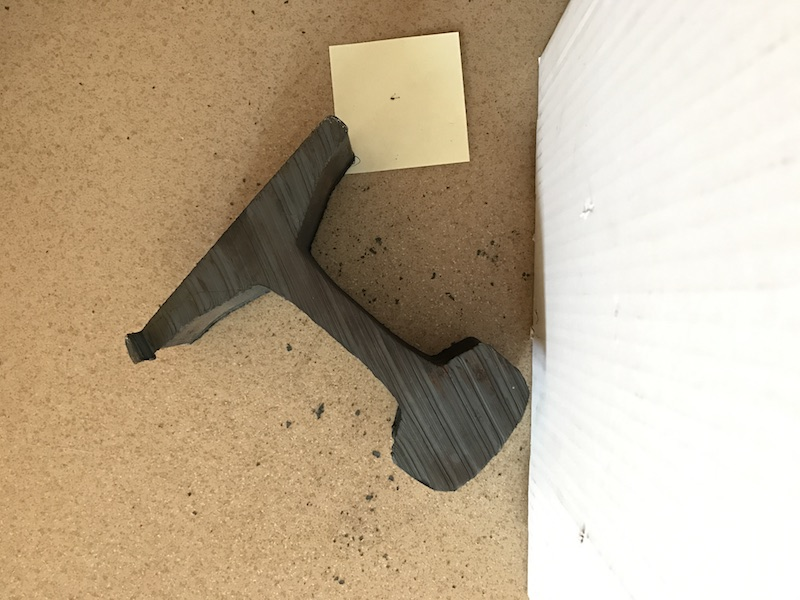
\includegraphics[width=0.45\textwidth]{images/example_rail}}
     \qquad
     \subfloat[]{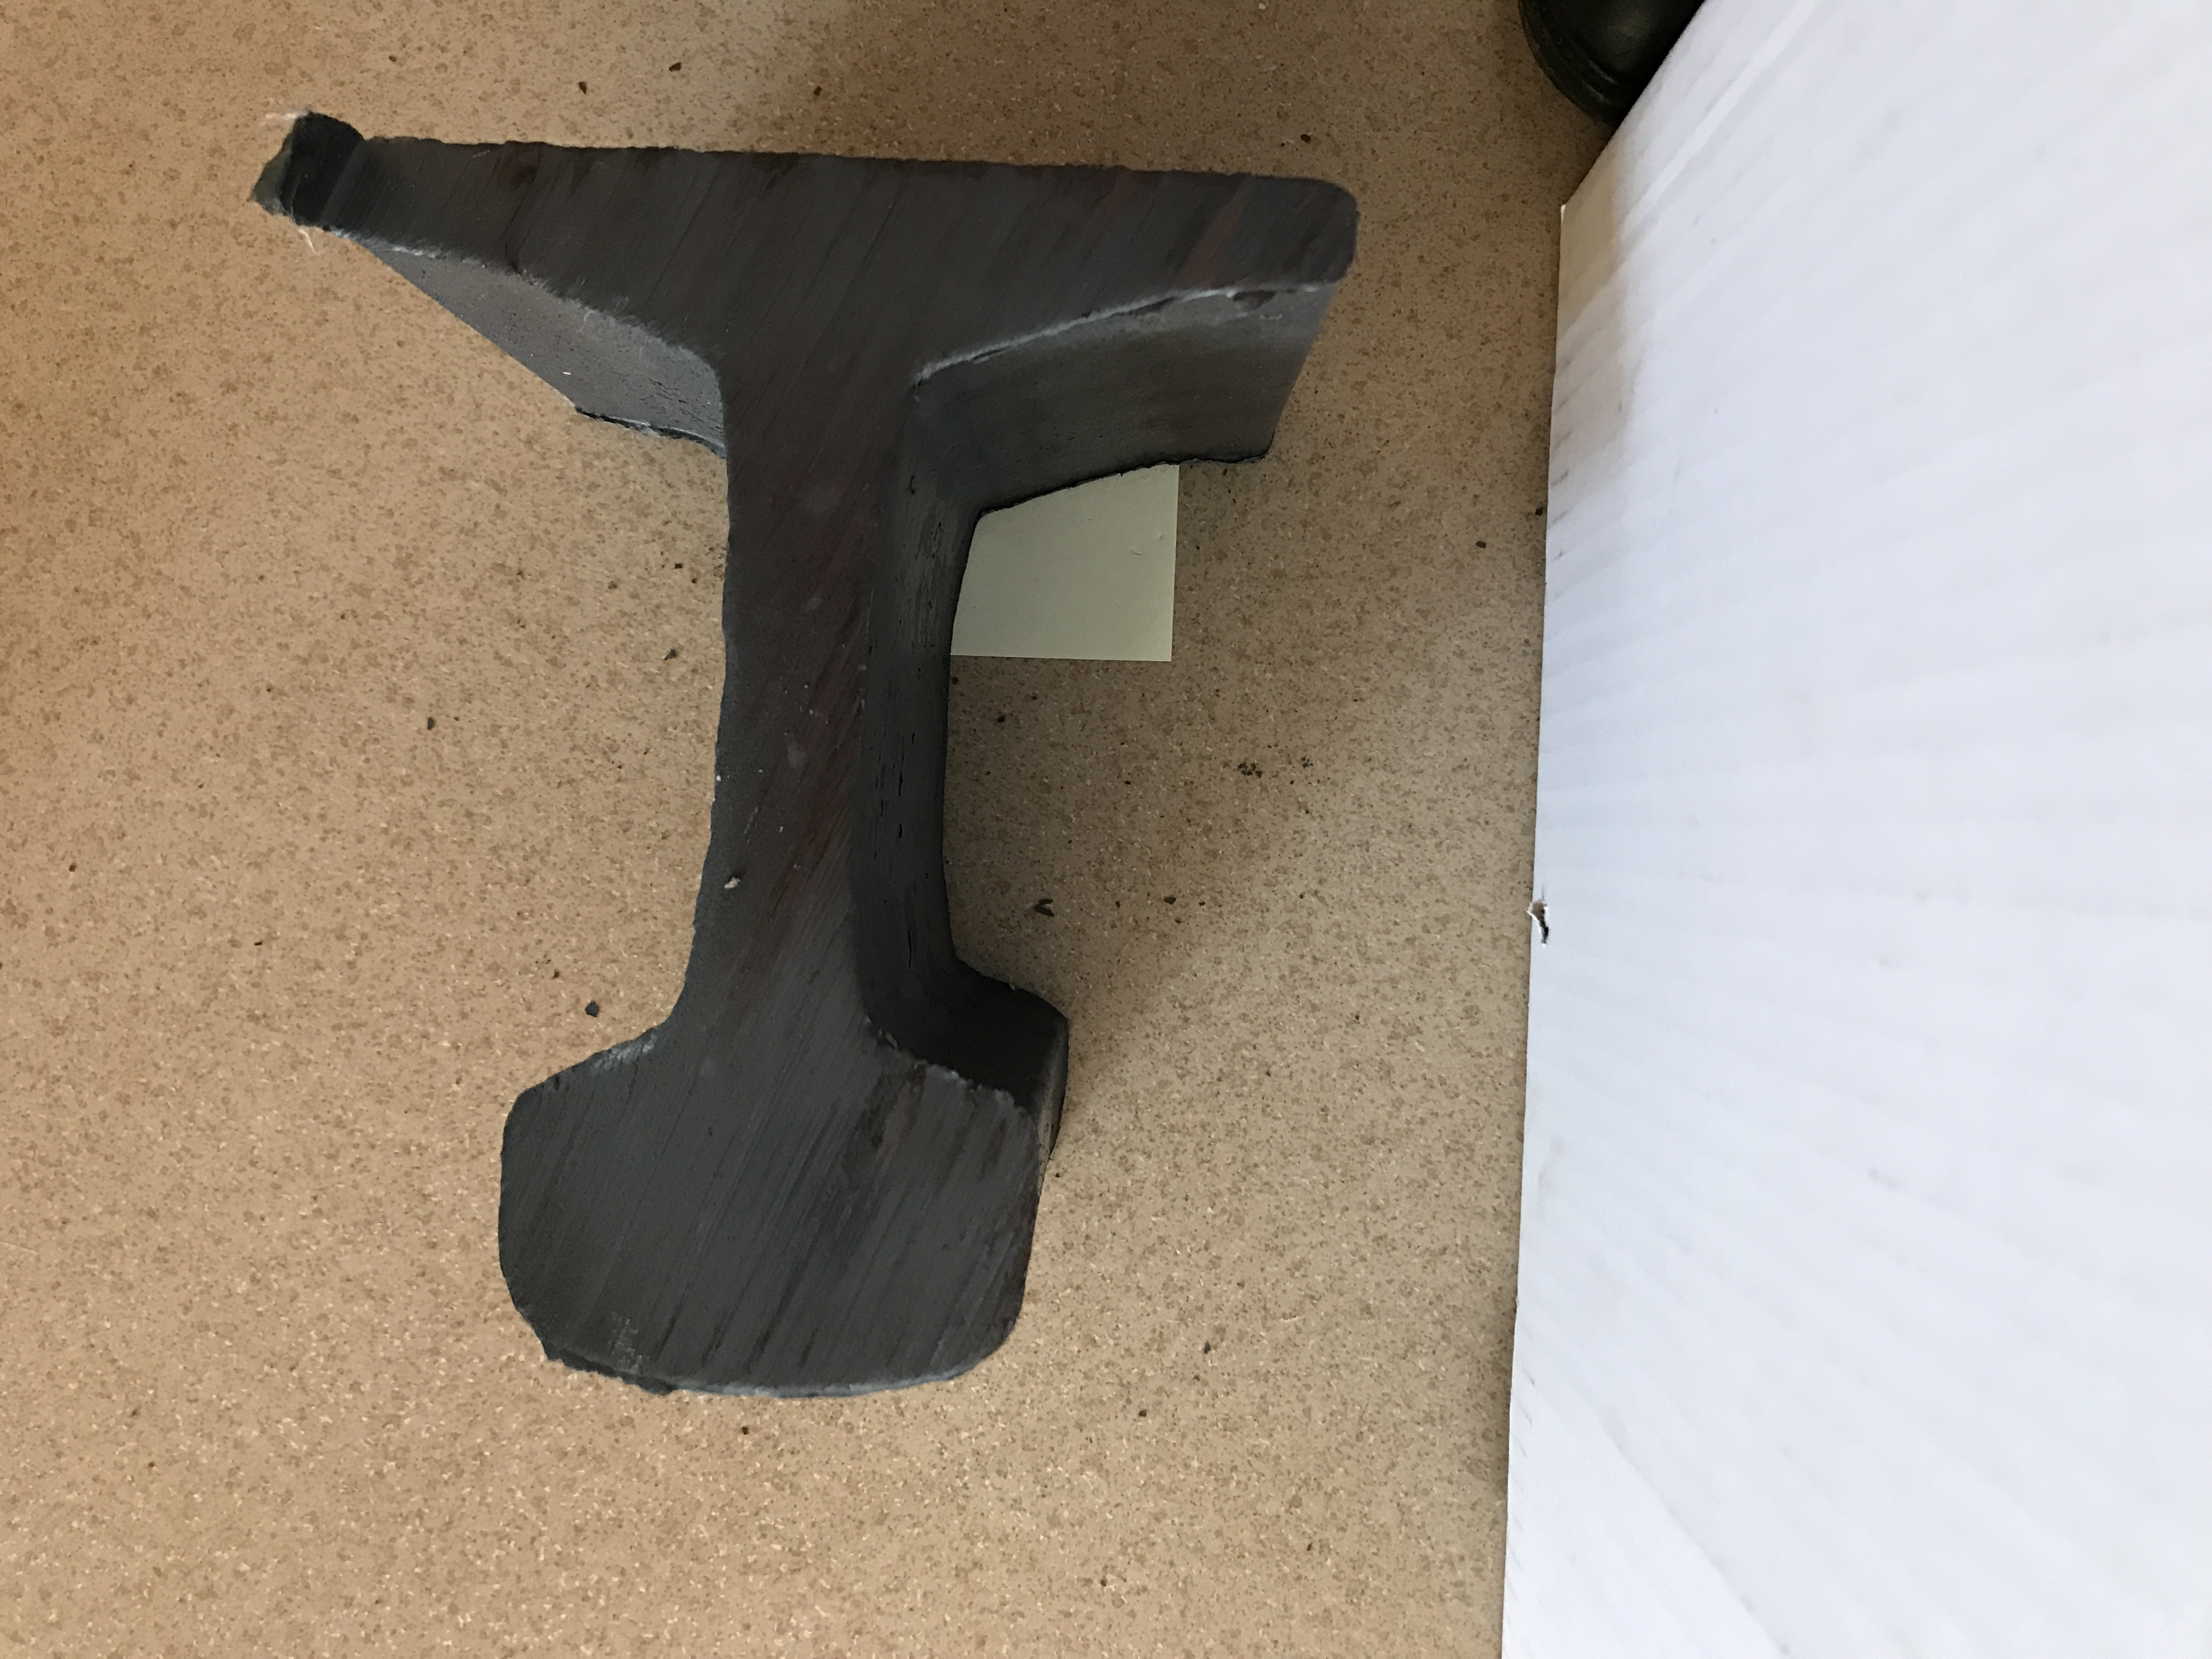
\includegraphics[width=0.45\textwidth]{images/example_rail_2}}
     \qquad
     \vfill
     \subfloat[]{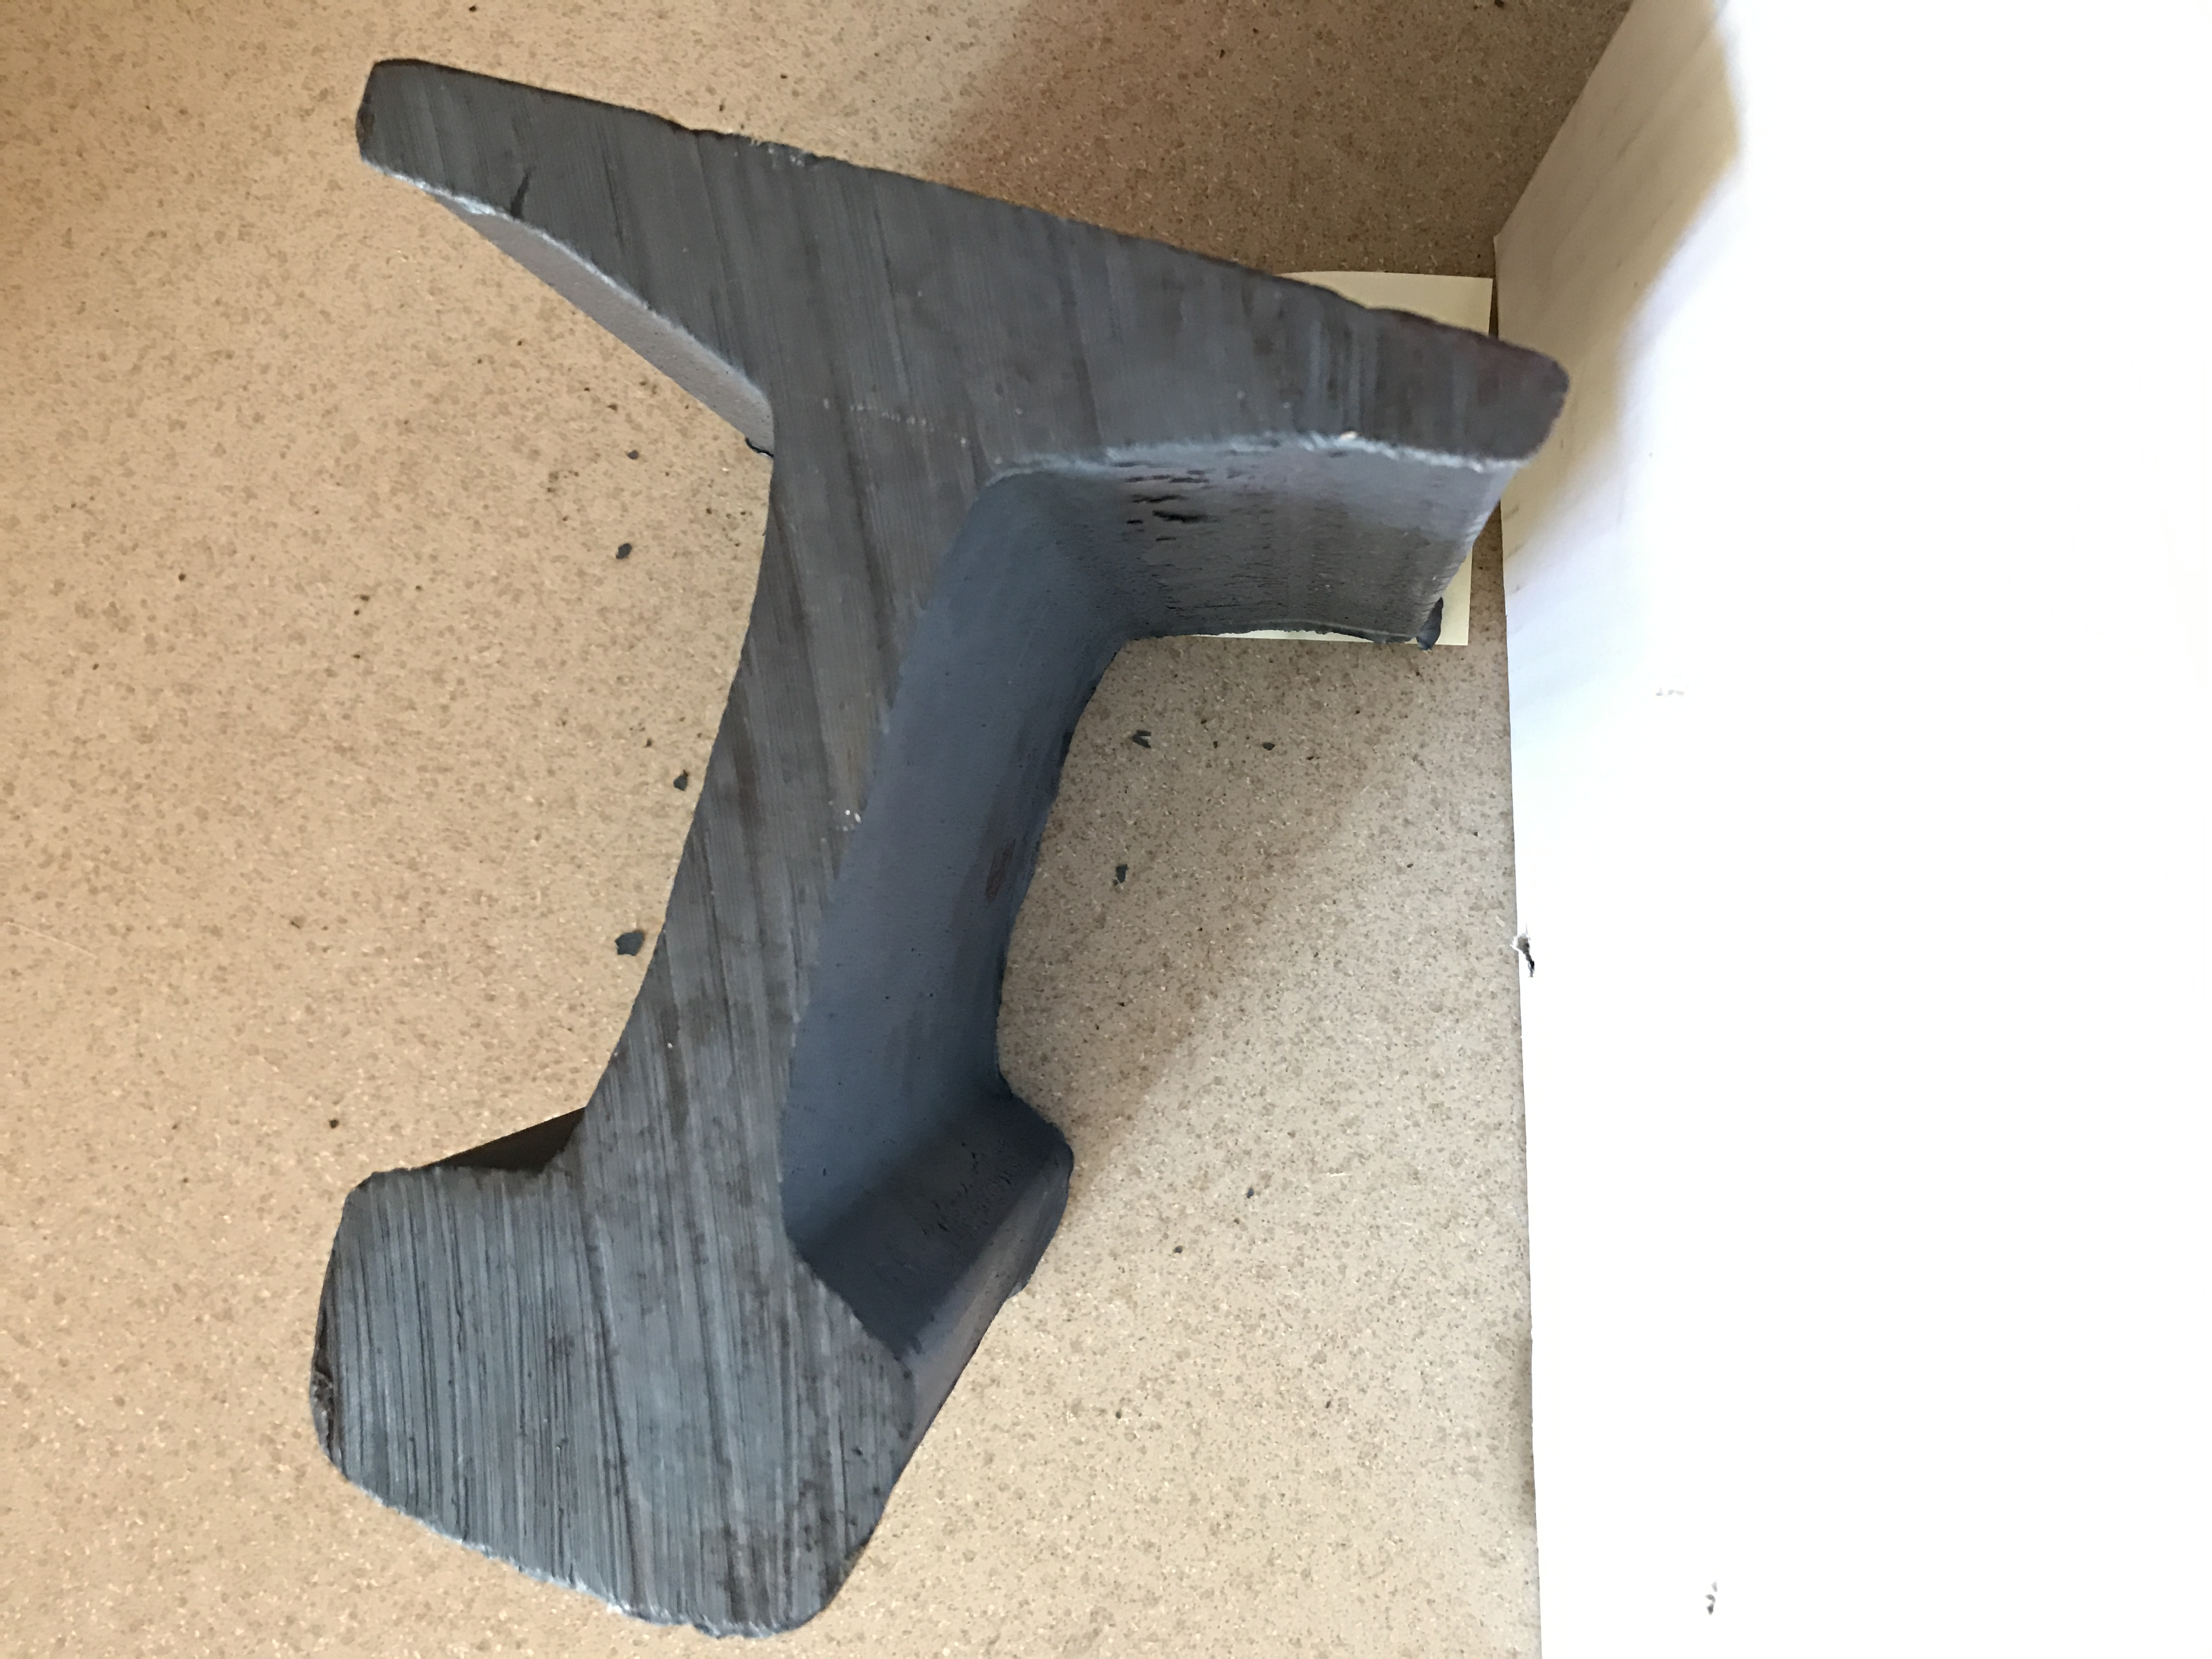
\includegraphics[width=0.45\textwidth]{images/example_rail_3}}
     \qquad
     \subfloat[]{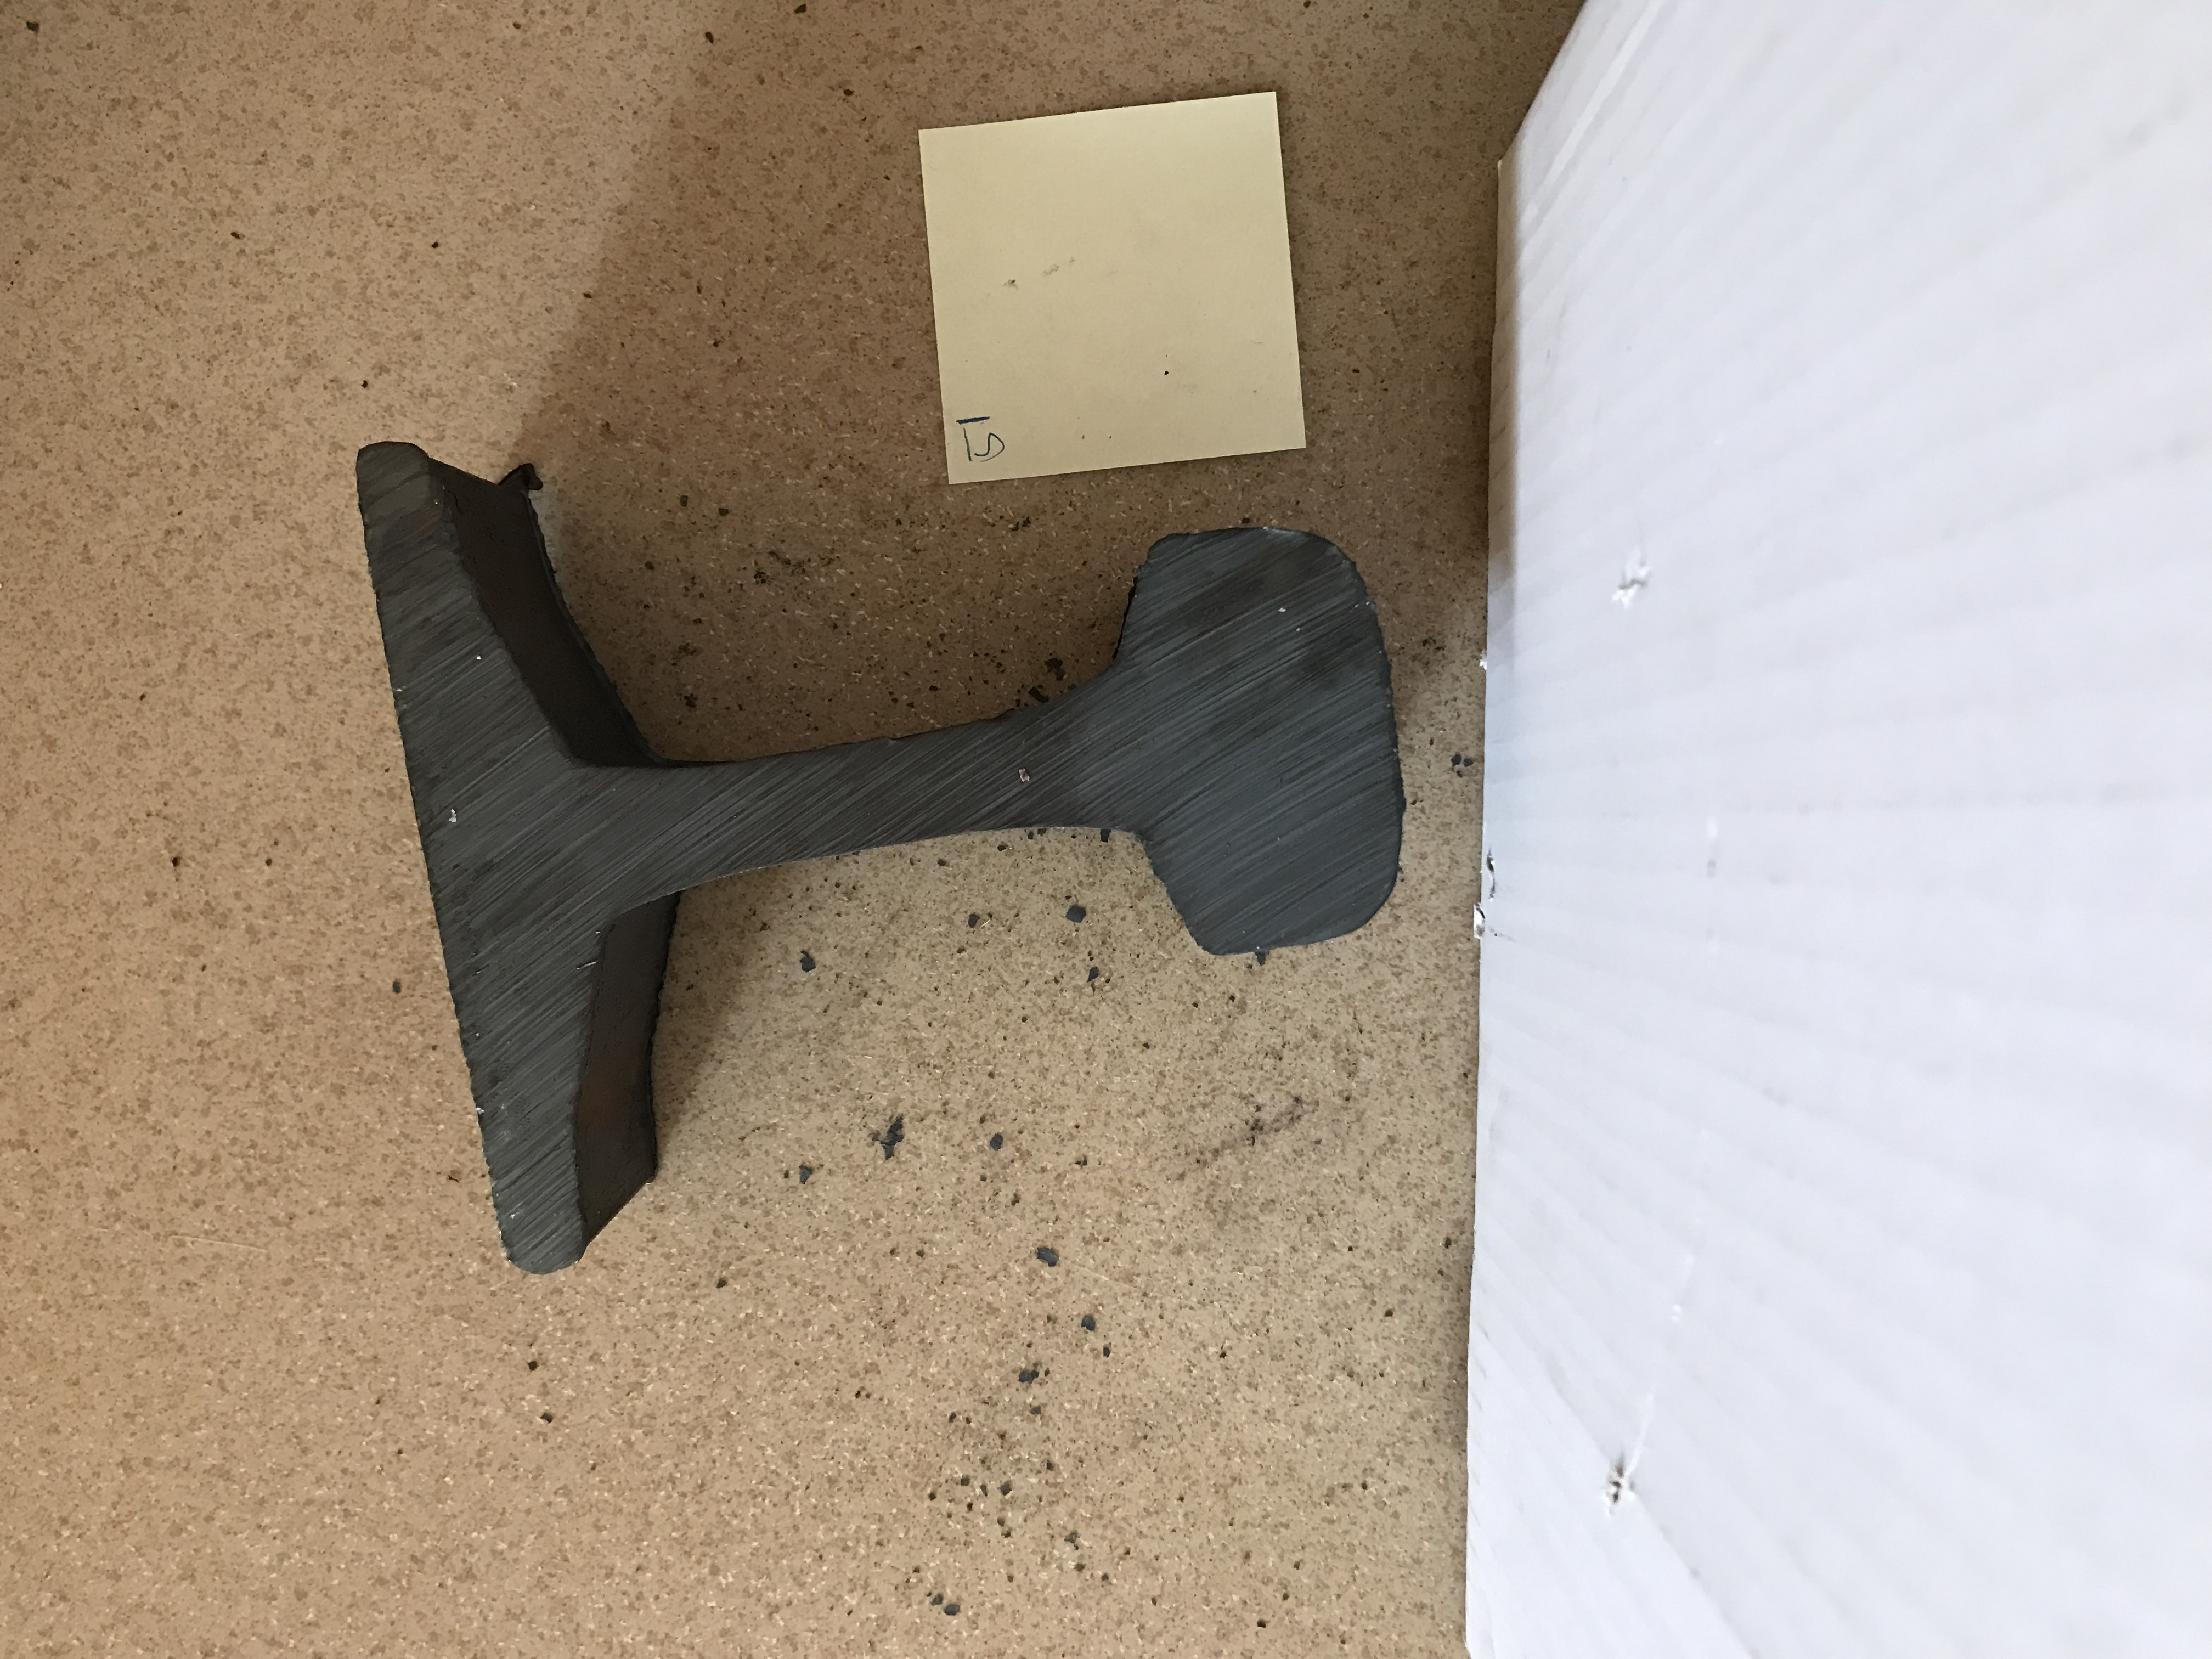
\includegraphics[width=0.45\textwidth]{images/example_rail_4}}
     \caption{Sample images of rails}
     \label{fig:different_lightning_conditions}
\end{figure}
 
\paragraph{}
However, provided the system will be implemented in production use, professional equipment will be installed (for example high quality camera) and maximal effort will be undertaken to ensure similar light conditions and background (ideally striking, monochromatic colour)

\section{Image Preprocessing}
\paragraph{Note}
The preprocessing of the image in our case means extracting from the input image just the parts that we are interested in and dropping the rest. Specifically, the only part of the rail that is of interest to us is the surface. So the desired output of this phase is an image containing only the surface of the rail with everything else as mono-coloured background (for example white). This is not the main focus of this thesis, so only a simplified, although giving very promising results, approach will be shown. It is likely that fine-tuning this algorithm would lead to having a fully working preprocessing stage.

\paragraph{Initial algorithm}
Before computing the "barcode" representation of the rail there is a couple of steps required to enable processing. The primary goal is to extract the shape of the split from the image, effectively ignoring everything else. Let us now look at the first attempt to approach this task using following techniques:

\begin{enumerate}
	\item Image thresholding (binary) - it is a function that for a given grayscale pixel\footnote{For color input, following RGB to grayscale transformation is used: \begin{equation*}Y \gets 0.299 * R + 0.587 * G + 0.114 * B\end{equation*}} assigns one of two values {A, B}. A is assigned to all of the pixels with value greater than some threshold value and B otherwise.
	$$
	threshold (pixel, T) = \begin{cases}
		A, pixel.value > T \\
		B, pixel.value <= T
	\end{cases}
	$$
	\item Finding contours - a function finding curves joining continuous points, having same colour or intensity
\end{enumerate}

\begin{algorithm}
	\begin{spacing}{1.5}
	\begin{algorithmic}[1]
		\Function{extract}{$grayscale$}
			\State $threshold \gets \textbf{cv2.threshold}(grayscale)$
			\State $contours \gets \textbf{cv2.findContours}(threshold)$
			\State $railContour \gets \textbf{maxArea}(contours)$
			\State $mask \gets \textbf{createMask}(railContour)$
			\State \textbf{return} $\textbf{cropImage}(grayscale, mask)$
		\EndFunction
	\end{algorithmic}
	\end{spacing}
	\caption{Extracting the shape of the split - first approach}
	\label{alg:extract_shape_1st}
\end{algorithm}

\paragraph{}
The Algorithm \ref{alg:extract_shape_1st} greatly simplifies the usage of OpenCV library - Open Source Computer Vision Library (\url{https://opencv.org/}), for which an overview is provided in \autoref{sec:opencv}. It does not provide any of the other required parameters for library functions and it also discards other return values. Function steps provide just the essential parts of the algorithm to present the idea. In line 2, a thresholding operation is applied to distinguish foreground and background on the image. Line 3, for previously obtained binary input, detects contours. Then, in line 4, a contour with maximal area is selected, from which a mask is created in line 5. That mask is then used, in line 6, to cut the foreground from the original input image. Please find high-level information about used functions:

\begin{enumerate}
	\item \textbf{maxArea()} - finds the contour with maximal area amongst ones provided as the parameter
	\item \textbf{createMask()} - creates a mask that includes the whole shape of contour (i.e. the edge and the interior) for a given contour
	\item \textbf{cropImage()} - to a given image applies a given mask, effectively cutting out just those pixels specified by the mask 
\end{enumerate}

\paragraph{}
The \textbf{cv2.} prefix in selected functions from Algorithm \ref{alg:extract_shape_1st} indicate that they come from second version of Python bindings for OpenCV. Please find excerpt from OpenCV documentation attached: \cite{opencv-docs}

\begin{enumerate}
	\item \textit{retval, dst} = \textbf{threshold}(\textit{src, thresh, maxval, type[, dst]}) - Applies a fixed-level threshold to each array element. The function returns the computed threshold value. \small{\begin{itemize}
		\item \textit{src} - input array
		\item \textit{thresh} - threshold value
		\item \textit{maxval} - max value to use with the binary and binary inverse type
		\item \textit{type} - thresholding type
		\item \textit{dst} - output array
	\end{itemize}}
	\item \textit{image, contours, hierarchy} = \textbf{findContours}(\textit{image, mode, method[, contours[, hierarchy[, offset]]]}) - Finds contours in a binary image \small{\begin{itemize}
		\item \textit{image} - source, an 8-bit single-channel image
		\item \textit{mode} - contour retrieval mode
		\item \textit{method} - contour approximation method
		\item \textit{contours} - detected contours
		\item \textit{hierarchy} - optional vector with information about the image topology
		\item \textit{offset} - optional offset by which every contour point is shifted
	\end{itemize}}
\end{enumerate}

\paragraph{Improved algorithm}
Further development of the preprocessing algorithm led to a little bit more complex series of steps presented in Algorithm \ref{alg:extract_shape_2nd}. Instead of converting whole RGB image to grayscale, the multi-channel array is split into separate single-channel arrays. Empirical experiments showed that for the given set of input images best results can be obtained when using just the red colour channel. The thresholding phase is now executed with threshold value computed from the histogram (first, peak value that corresponds to the rail is found and then after performing simple algebraic operations is used to obtain the value). The thresholding process returns a binary image where white colour denotes area that is most likely a part of the rail and a black colour otherwise. Such a binary image then undergoes a series of corresponding image blurring (using median blur filter) and morphological opening (which is a series of erosions followed by dilations). To complete the process and fill some gaps that may have appeared in some of the previous phases, a fill holes procedure is applied.

\begin{algorithm}
	\begin{spacing}{1.5}
	\begin{algorithmic}[1]
		\Function{extract}{$image$}
			\State $redChannel \gets$ R channel from the $image$
			\State $railPeak \gets$ rail peak from histogram of $redChannel$
			\State $threshold \gets \textbf{threshold}(redChannel, railPeak)$
			\State $blur \gets \textbf{cv2.medianBlur}(threshold)$
			\For{$i \gets 0\ \textbf{to}\ repetitions$}
				\State $opening \gets \textbf{open}(blur)$
				\State $blur \gets \textbf{cv2.medianBlur}(opening)$
			\EndFor
			\State $filled \gets \textbf{fillHoles}(blur)$
			\State $contours \gets \textbf{cv2.findContours}(filled)$
			\State $railContour \gets \textbf{maxArea}(contours)$
			\State $mask \gets \textbf{createMask}(railContour)$
			\State \textbf{return} $\textbf{cropImage}(grayscale, mask)$
		\EndFunction
	\end{algorithmic}
	\end{spacing}
	\caption{Extracting the shape of the split - improved approach}
	\label{alg:extract_shape_2nd}
\end{algorithm}

\paragraph{}
Let us now look at the Algorithm \ref{alg:extract_shape_2nd}. In line 2, red channel is taken from the input image. Next, in line 3, a thresholding value is selected as the most-frequently occurring red value and is used in line 4 to perform the actual threshold. In line number 5 a blurring operation is applied to the binary output of thresholding. The loop in lines 6 to 9 performs repetitive opening and blurring of binary image. After the loop finishes, any holes that might have occurred, are treated as foreground, in line 10. Lines 11-14 repeat last steps from previous Algorithm \ref{alg:extract_shape_1st}.

\paragraph{}
Please find excerpt from OpenCV documentation, for function from Algorithm \ref{alg:extract_shape_2nd}, attached: \cite{opencv-docs}

\begin{enumerate}
	\item \textit{dst} = \textbf{medianBlur}(\textit{src, ksize[, dst]}) - Blurs an image using the median filter. \small{\begin{itemize}
		\item \textit{src} - input
		\item \textit{dst} - destination array of the same size and type as src
		\item \textit{ksize} - aperture linear size; it must be odd and greater than 1
	\end{itemize}}
\end{enumerate}

\begin{figure}[H]
     \centering
     \subfloat[Before]{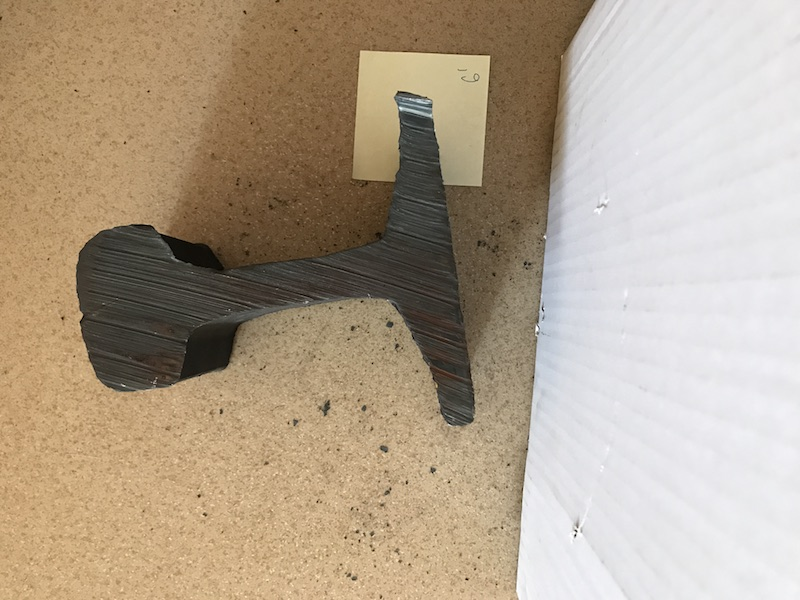
\includegraphics[width=0.45\textwidth]{images/good_before_preprocessing}}
     \qquad
     \subfloat[After thresholding]{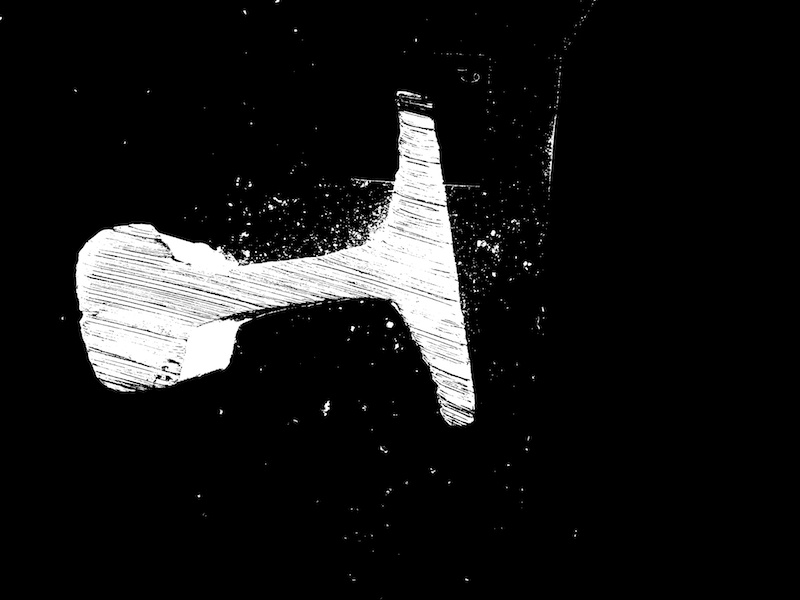
\includegraphics[width=0.45\textwidth]{images/good_after_thresholding}}
     \qquad
     \vfill
     \subfloat[After opening and blurring]{
\includegraphics[width=0.45\textwidth]{images/good_after_opening_and_blurring}}
     \qquad
     \subfloat[Shape detected]{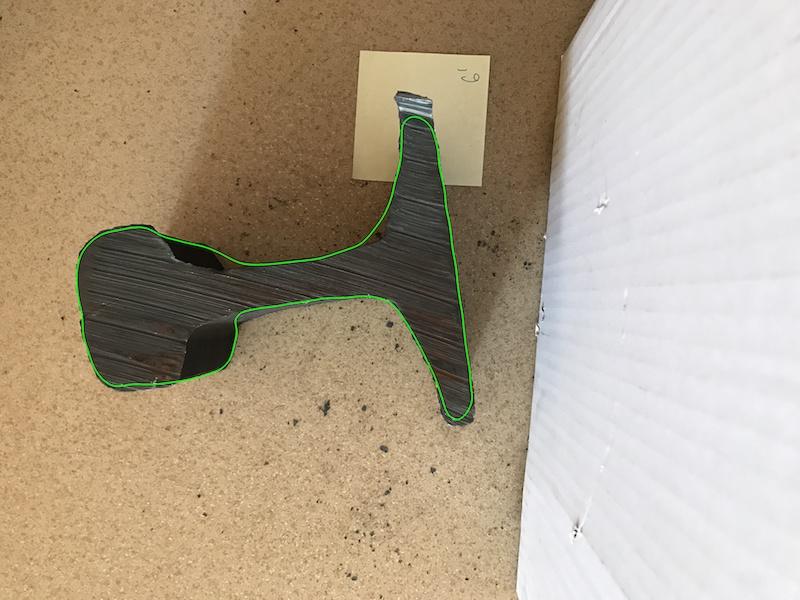
\includegraphics[width=0.45\textwidth]{images/good_after_preprocessing}}
     \caption{Stages of preprocessing - successful}
     \label{fig:preprocessing}
\end{figure}

\section{Image Processing}
\paragraph{}
Given that the main purpose of the thesis is the identification of foundry details, we can skip further contemplation of the preprocessing phase. The shape detection and extraction can be treated as a separate algorithm that needs to be developed and fine-tuned.

\paragraph{}
Assuming we have such an algorithm and thus a successful preprocessing phase, in the actual computing phase the input images contain only the surfaces of the rails (see figure \ref{fig:preprocessing_outputs}).

\paragraph{Note}
The actual input images for the processing phase, as shown in figure \ref{fig:preprocessing_outputs}, were prepared manually. It was done using free and open source image editor GIMP (\url{https://www.gimp.org/}), by utilizing its' \textit{Free Select Tool}.

\begin{figure}[H]
     \centering
     \subfloat[]{\fbox{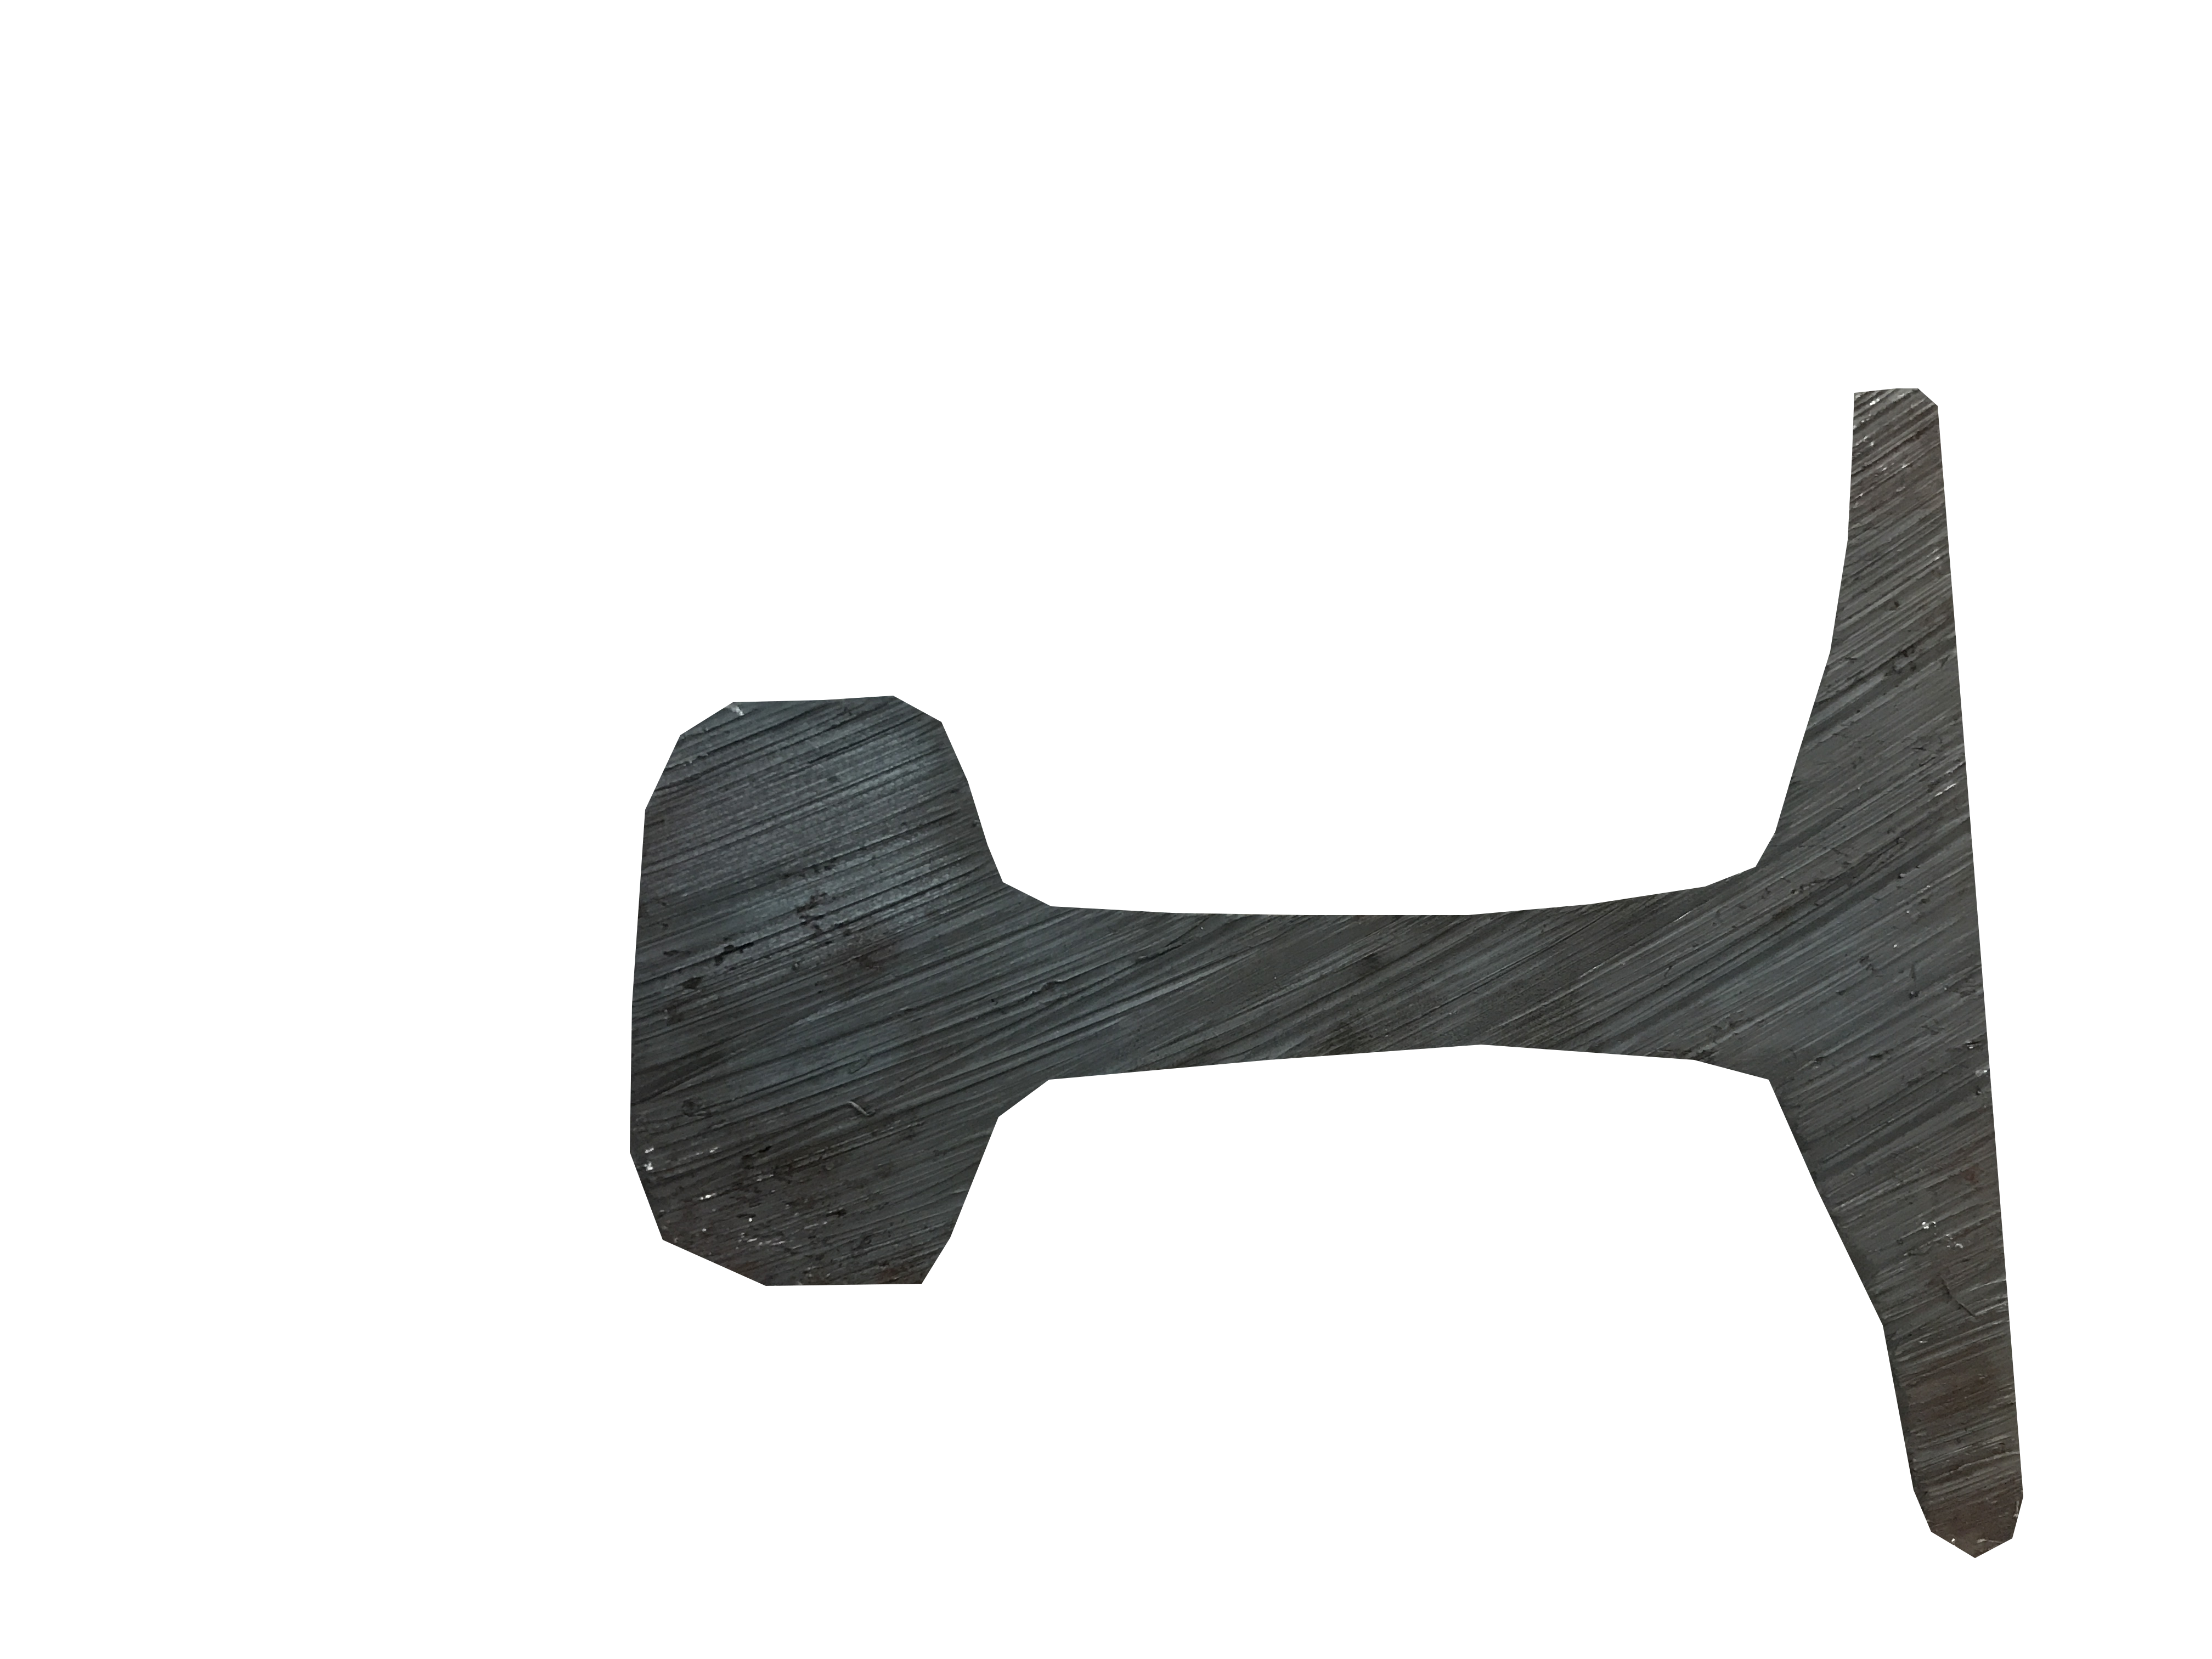
\includegraphics[width=0.45\textwidth]{images/preprocessed_1}}}
     \qquad
     \subfloat[]{\fbox{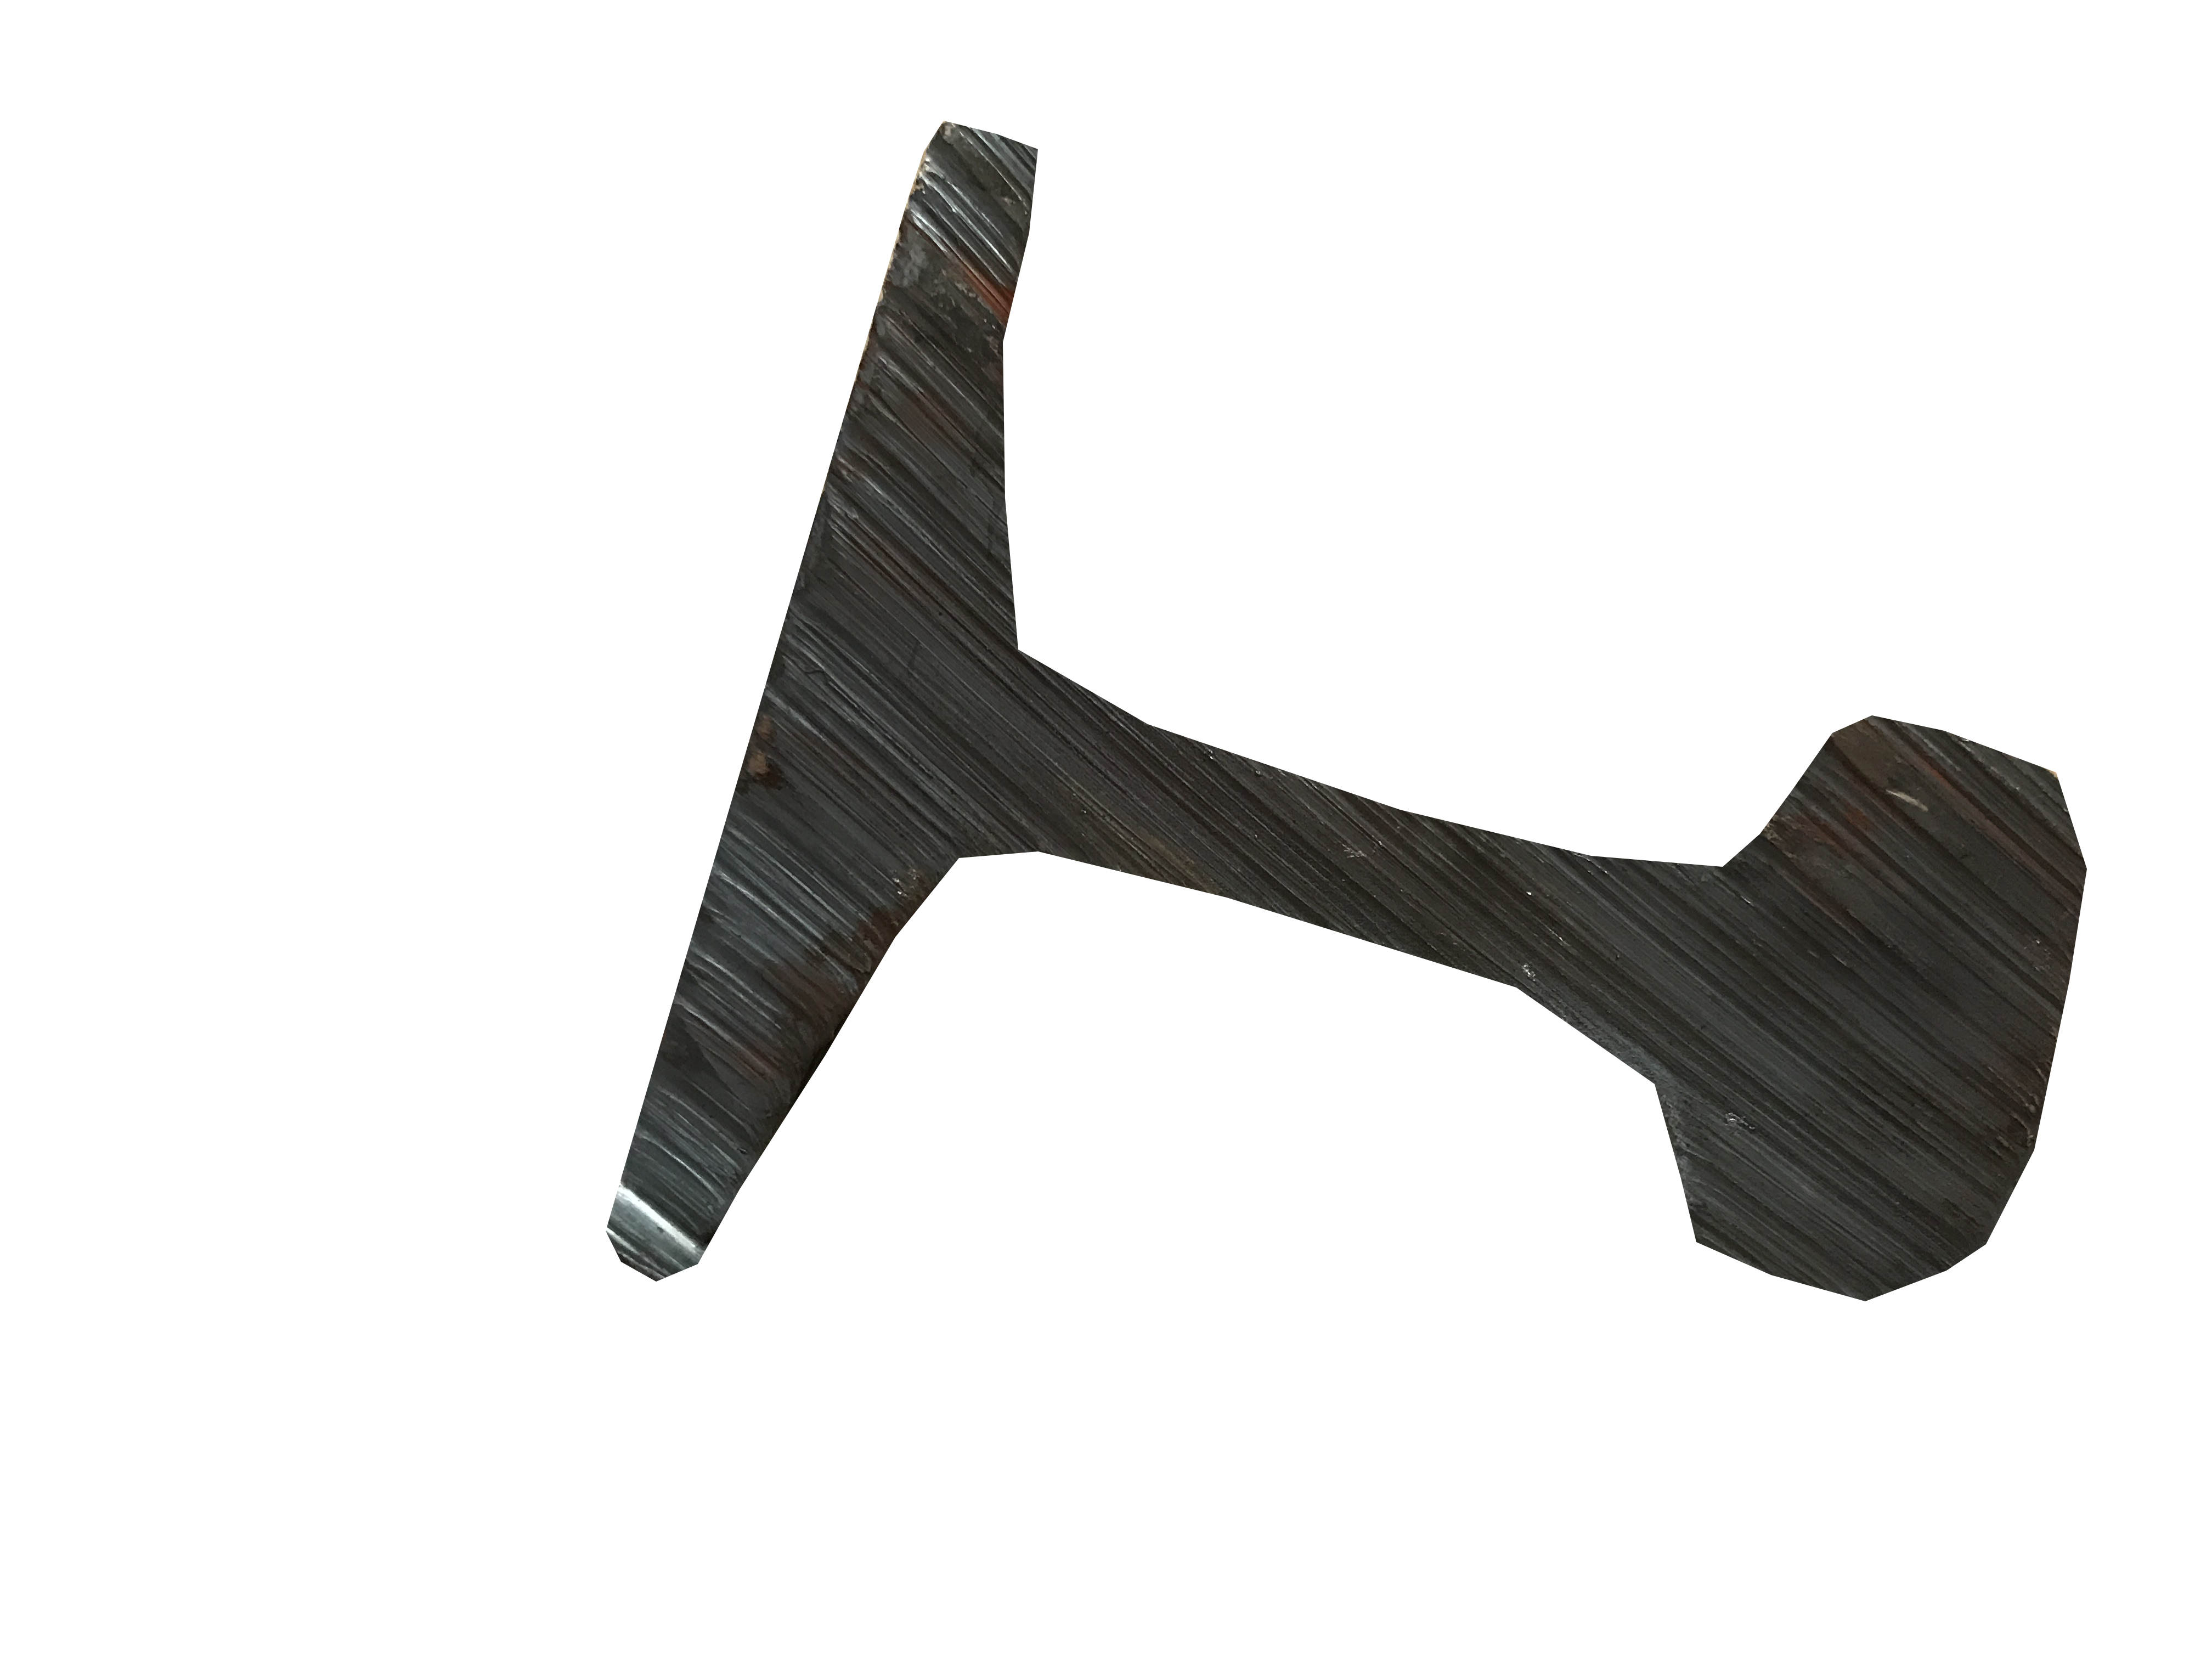
\includegraphics[width=0.45\textwidth]{images/preprocessed_2}}}
     \qquad
     \vfill
     \subfloat[]{\fbox{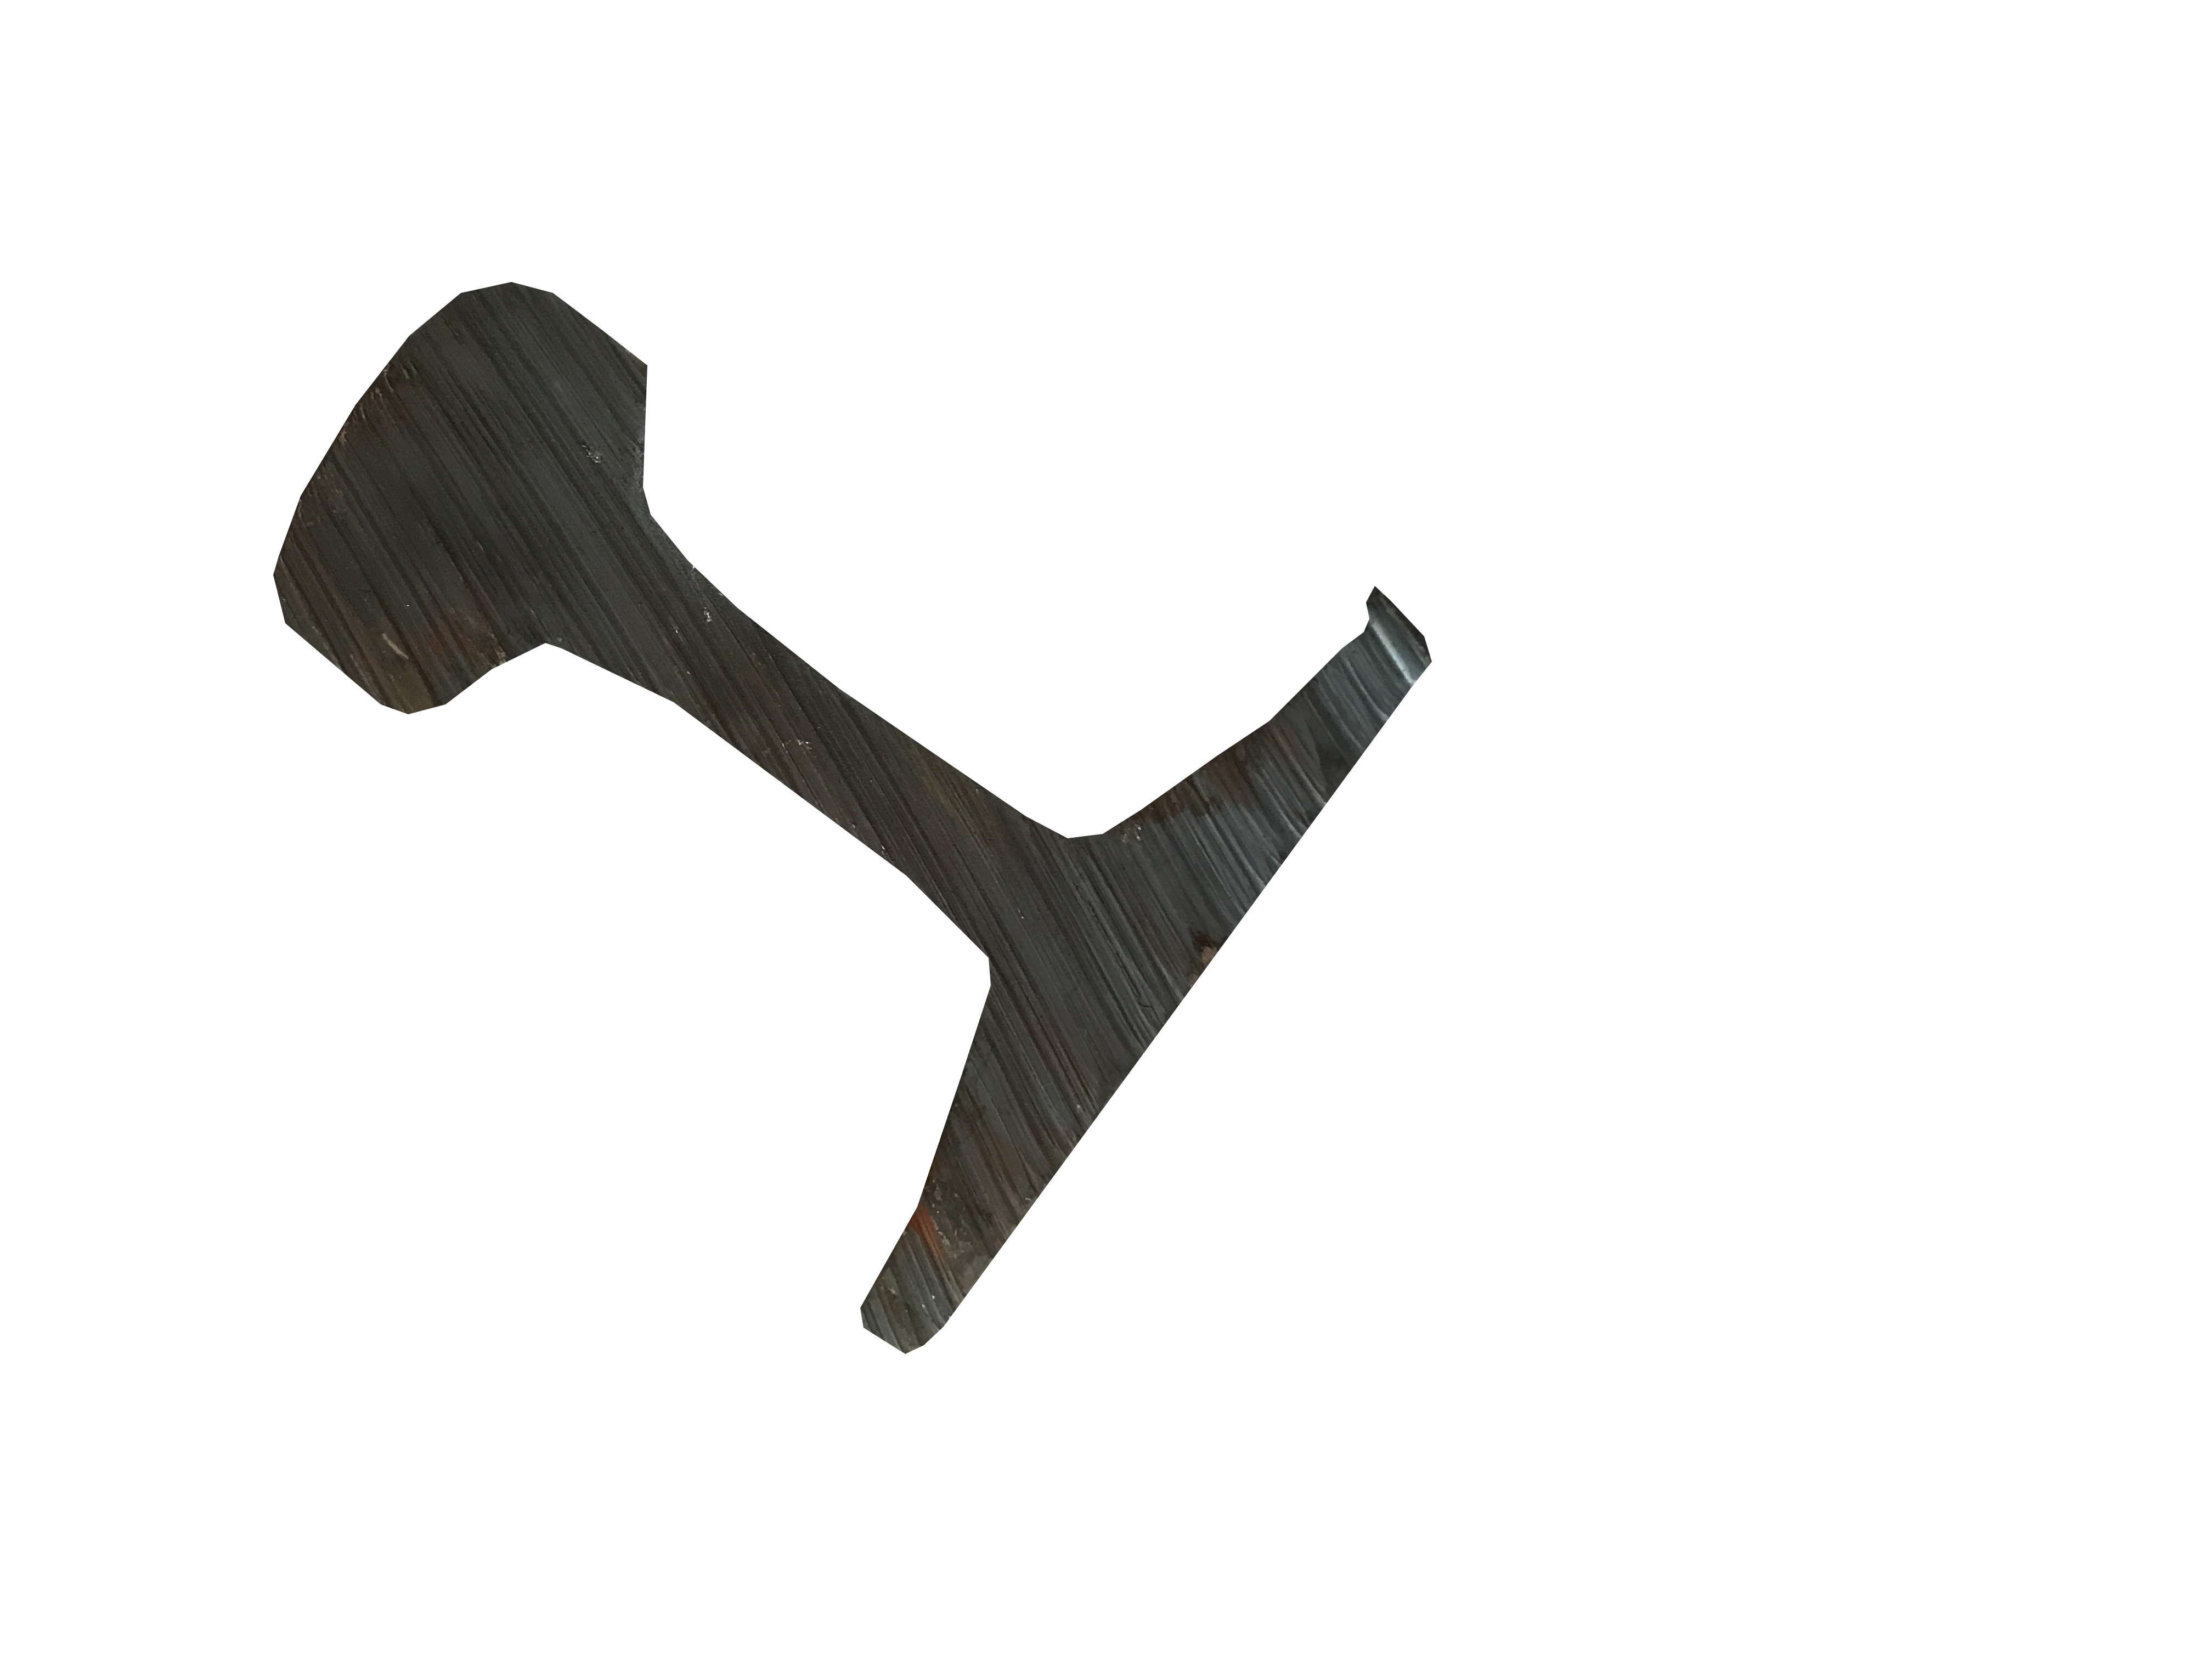
\includegraphics[width=0.45\textwidth]{images/preprocessed_3}}}
     \qquad
     \subfloat[]{\fbox{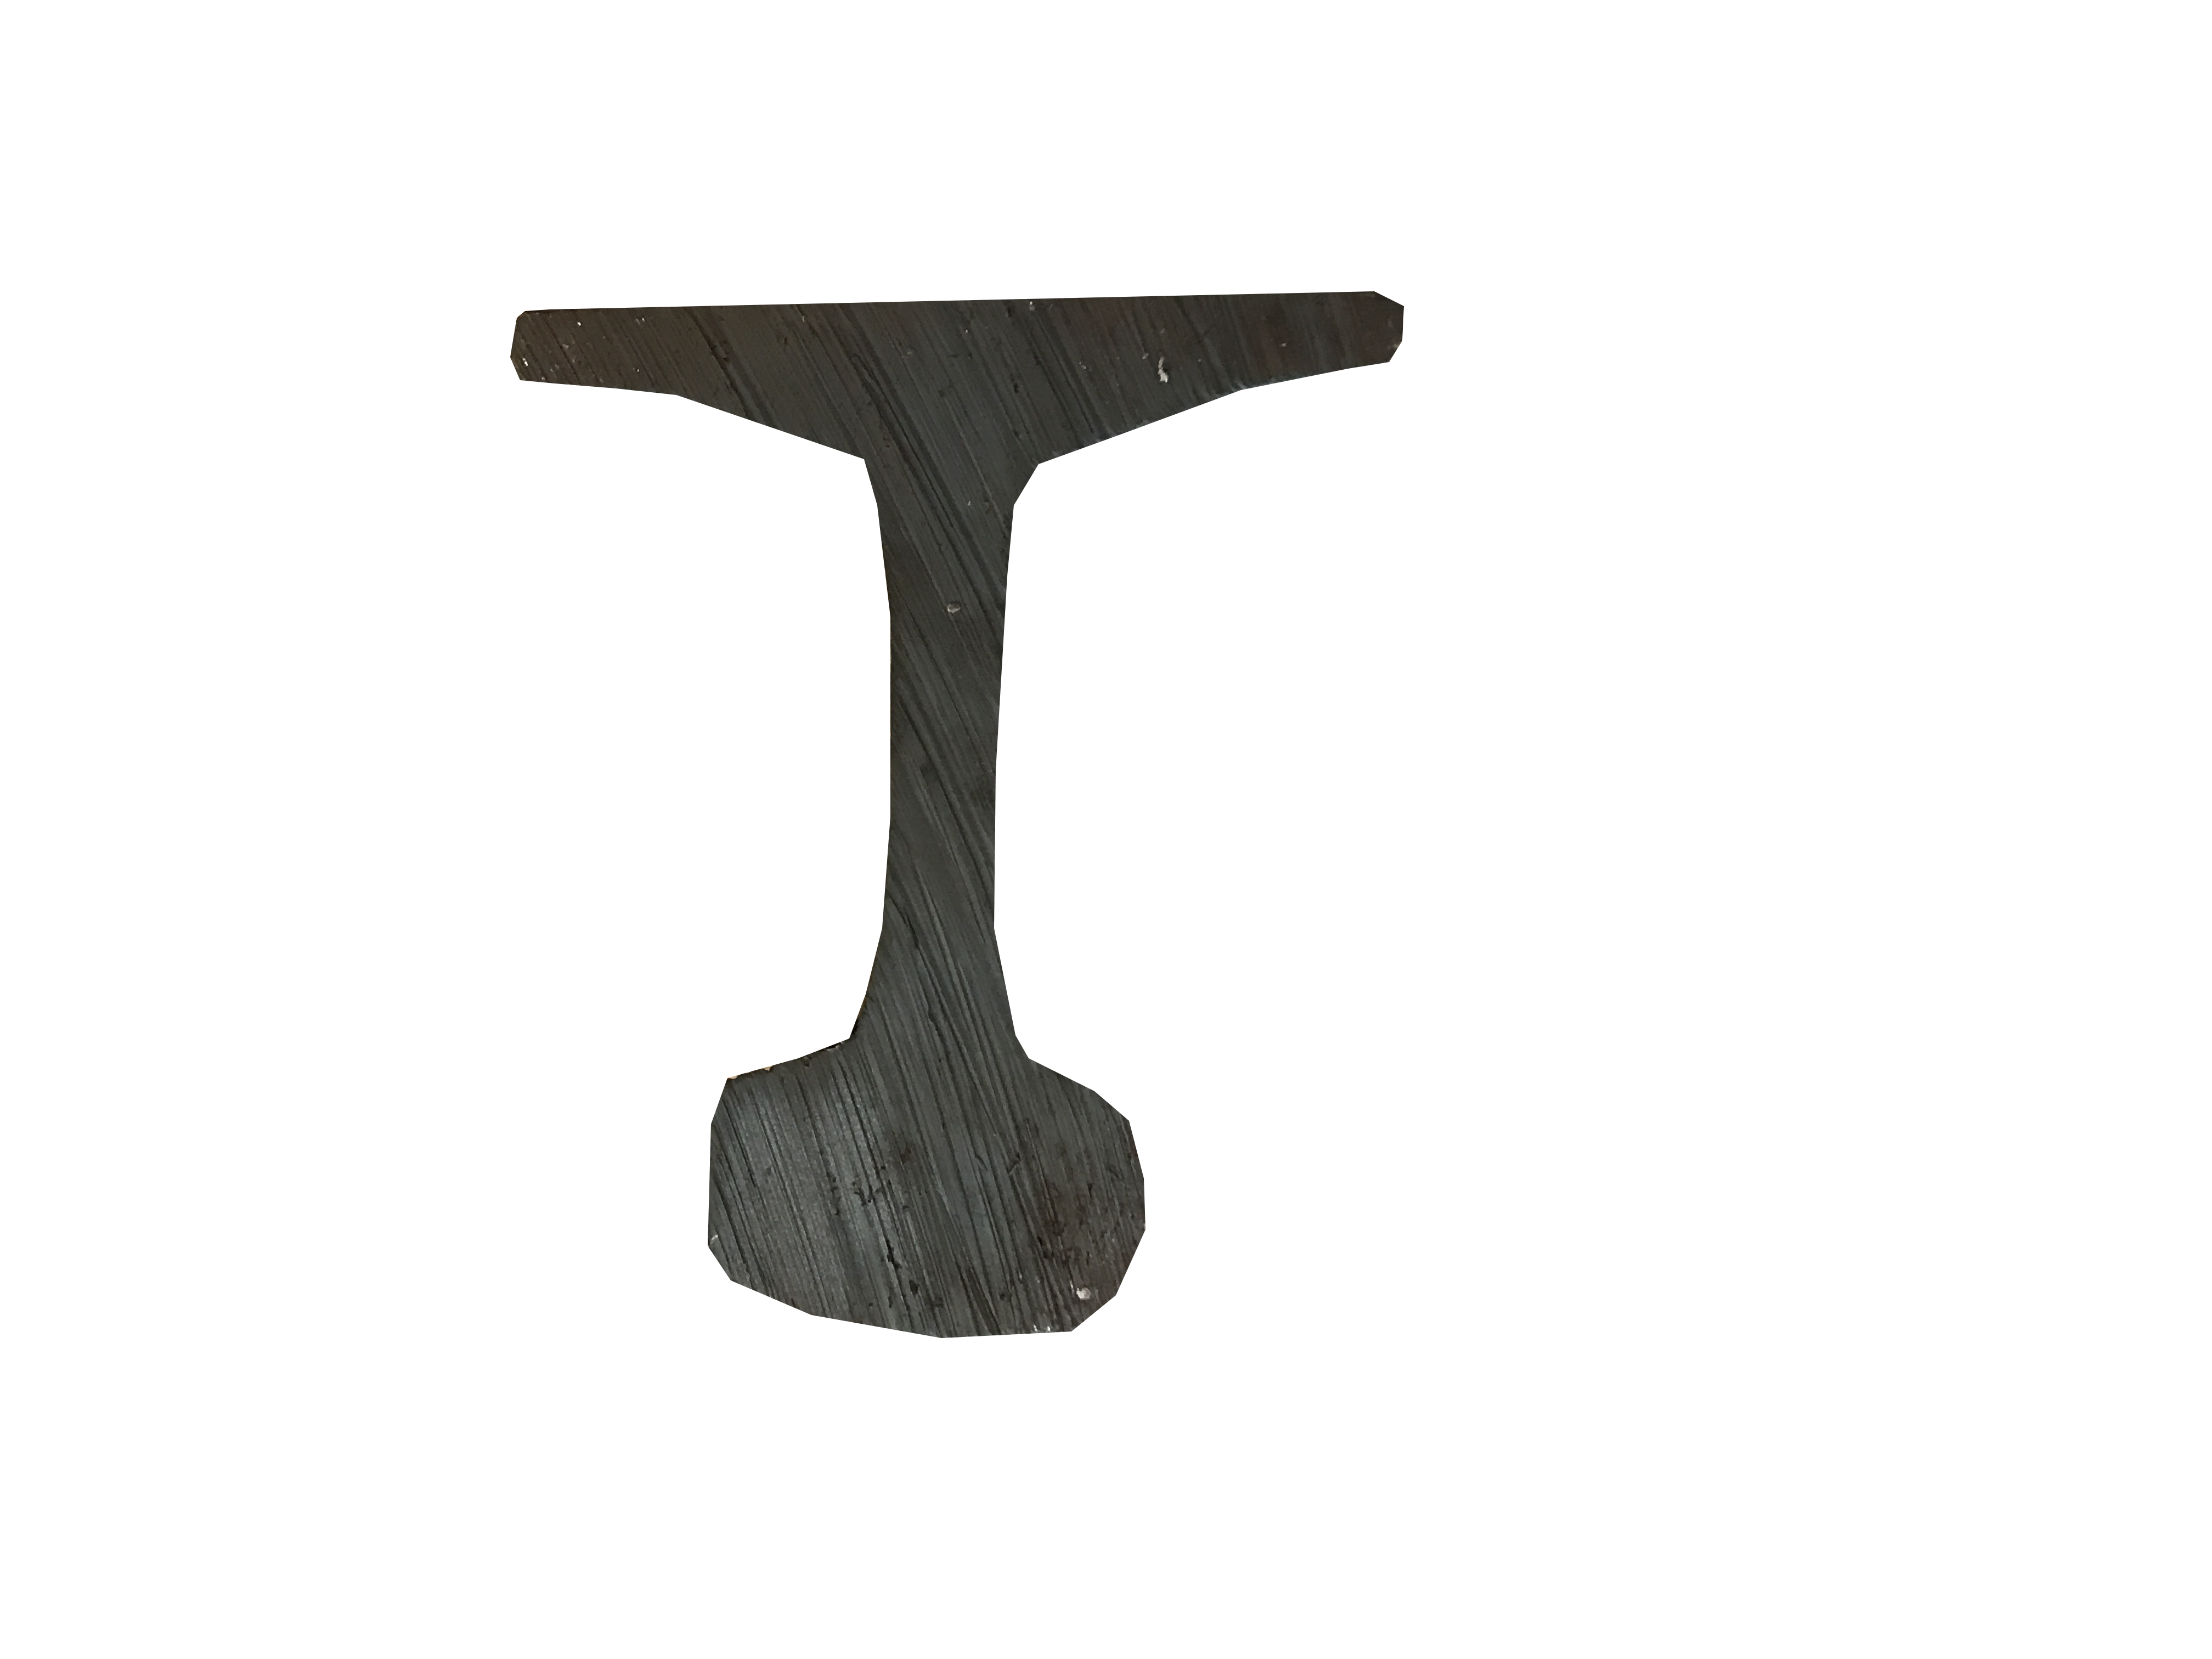
\includegraphics[width=0.45\textwidth]{images/preprocessed_4}}}
     \caption{Preprocessing outputs}
     \label{fig:preprocessing_outputs}
\end{figure}

\paragraph{}
In order to reduce complexity of the processing phase, a need to find some optimizations emerged. One of the solutions that was under investigation was to scale the image down - but it led to more noise being introduced and thus the comparison results being less accurate. Experiments and development of the processing algorithm showed that the most significant part for the comparison of barcodes lies in the upper half of the rail surface - the "ellipse-shaped" part of it. It is due to the fact that this area is the most stable across all of the images in terms of the barcode readability and consistency. This is why the lower part of the image is actually dropped altogether from the analysis.

\paragraph{}
Let us now look at the Algorithm \ref{alg:comparing} for comparing two images. Lines 2 and 3 are responsible for taking just the upper half of both input images. Next, in lines 4 and 5, dominant angles for both upper halves are found. The conditional expression in lines 6-9 detects a difference in dominant angles higher than the admissible threshold and immediately signals that the two images show different rails if this threshold is crossed. In lines 9 and 10 both upper halves are rotated so that the barcode is perpendicular to the X-axis. In line 11 a function is called to find the maximal comparison result of the two rotated images. It performs also some slight rotations to accommodate for some minor differences in detected dominant angles. Finally, in line 12, the returned result is verified and if it is satisfactory, then we assume the original input images show the same rail. Otherwise, the output is negative. 

\begin{algorithm}
	\begin{spacing}{1.5}
	\begin{algorithmic}[1]
		\Function{compare}{$image1, image2$}
			\State $image1\_up \gets$ upper half from the $image1$
			\State $image2\_up \gets$ upper half from the $image2$
			
			\State $angle1 \gets \textbf{dominantAngle}(image1\_up)$
			\State $angle2 \gets \textbf{dominantAngle}(image2\_up)$
			
			\If{$\textbf{abs}(angle1 - angle2) > \textbf{THRESHOLD\_ANGLE}$}
				\State \textbf{return} FALSE
			\EndIf
			
			\State $rotated1 \gets \textbf{rotate}(image1\_up, angle1)$
			\State $rotated2 \gets \textbf{rotate}(image2\_up, angle2)$
			
			\State $result \gets \textbf{findMaxComparisonResult}(rotated1, rotated2)$
			\State \textbf{return} $result > \textbf{THRESHOLD\_COMPARISON}$
		\EndFunction
	\end{algorithmic}
	\end{spacing}
	\caption{Comparing two preprocessed rail images}
	\label{alg:comparing}
\end{algorithm}

\begin{itemize}
	\item \textbf{dominantAngle(image)} - this function finds the most frequent angle amongst the lines that create the pattern. The image first undergoes Canny Edge detection, so line detection algorithm can later be used. It does so by utilising OpenCV's \textbf{HoughLinesP}\footnote{It works similar to the standard Hough line transformation, that is described in \autoref{sec:hough_lines} with two important differences. The lines are represented as start and end points. The second difference is the ability to specify the minimum length of a line segment and the separation between collinear segments required for the algorithm not to join them into a single longer segment.\cite{learning-opencv-3}} function from which those angles can be computed, rounded and the dominant one is selected. The pseudocode and some explanation for this algorithm is provided later in this chapter.
	\item \textbf{rotate(image, angle)} - this function simply rotates the image by a given angle. It is used to point the lines that form the patter perpendicular to X-axis.
	\item \textbf{findMaxComparisonResult(image1, image2)} - this function is returning the final comparison result. In order to alleviate some differences in the dominant angle resulting in slightly different rotations, this function itself also does some minor rotations for first of the images and each such rotation is being compared with the second image. Maximum value of those comparisons is then returned as the final value.
\end{itemize}

\paragraph{}
Algorithm \ref{alg:dominant_angle} detects the most-frequently occurring angle among the lines on the rail's surface. In line 2 light is equalized, then, in line 3, a color space conversion to grayscale is applied. Such an image is passed to Canny function for edge detection in line 4. Next an accumulator array for detected angles is created in line 5 and, in line 6, probabilistic Hough lines transform is applied to the detected edges. The loop in lines 7 through 12, for each line that was reported from the Hough transform, the angle is computed and added to the accumulator. In line 13, a histogram of the angles is created, and the dominant one is chosen in lines 14 and 15.

\begin{algorithm}
	\begin{spacing}{1.5}
	\begin{algorithmic}[1]
		\Function{dominantAngle}{$color\_image$}
			\State $equalized \gets \textbf{equalizeLight}(color\_image)$
			\State $gray \gets \textbf{cv2.cvtColor}(equalized)$
			\State $edges \gets \textbf{cv2.Canny}(gray)$
			\State $angles \gets []$
			\State $lines \gets \textbf{cv2.HoughLinesP}(edges)$
			\For{$line \gets lines$}
				\State $x1, y1, x2, y2 \gets line$
				\State $a \gets $ slope of $x1, y1, x2, y2$
				\State $angle \gets$ get angle for $slope$
				\State $angles.append(angle)$
			\EndFor
			\State $histogram \gets \textbf{np.histogram}(angles, bins=360, range=(0, 180))$
			\State $convolution \gets \textbf{np.convolve}(hist, \textbf{np.ones}(6))$
			\State \textbf{return} $\textbf{np.argmax}(convolution) / 2.0$
		\EndFunction
	\end{algorithmic}
	\end{spacing}
	\caption{Finding the dominant angle}
	\label{alg:dominant_angle}
\end{algorithm}

\paragraph{}
Please find excerpt from OpenCV documentation, for functions from Algorithm \ref{alg:dominant_angle}, attached: \cite{opencv-docs}

\begin{enumerate}
	\item \textit{dst} = \textbf{cvtColor}(\textit{src, code[, dst[, dstCn]]}) - Converts an image from one color space to another. \small{\begin{itemize}
		\item \textit{src} - input image
		\item \textit{dst} - output image of the same size and depth as src
		\item \textit{code} - color space conversion code
		\item \textit{dstCn} - number of channels in the destination image
	\end{itemize}}
	\item \textit{edges} = \textbf{Canny}(\textit{image, threshold1, threshold2[, edges[, apertureSize[, L2gradient]]]}) - Finds edges in an image using the Canny algorithm. \small{\begin{itemize}
		\item \textit{image} - source, an 8-bit single-channel image
		\item \textit{edges} - output edge map
		\item \textit{threshold1} - first threshold for the hysteresis procedure
		\item \textit{threshold2} - second threshold for the hysteresis procedure
		\item \textit{apertureSize} - aperture size for the Sobel operator
		\item \textit{L2gradient} - a flag, indicating whether a more accurate $L_2$ norm
	\end{itemize}}
	\item \textit{lines} = \textbf{HoughLinesP}(\textit{image, rho, theta, threshold[, lines[, minLineLength[, maxLineGap]]]}) - Finds line segments in a binary image using the probabilistic Hough transform. \small{\begin{itemize}
		\item \textit{image} - source, an 8-bit single-channel image
		\item \textit{lines} - output vector of lines
		\item \textit{rho} - distance resolution of the accumulator in pixels
		\item \textit{theta} - angle resolution of the accumulator in radians
		\item \textit{threshold} - accumulator threshold parameter
		\item \textit{minLineLength} - min line length
		\item \textit{maxLineGap} - max allowed gap between points on the same line to link them	
	\end{itemize}}
\end{enumerate}

\paragraph{}
In order to accommodate for some relic peaks, it is actually not the most frequently occurring angle but it is accumulatively taken within 3 degrees and only then the max is picked.

\begin{figure}[H]
     \centering
     \subfloat[Original input]{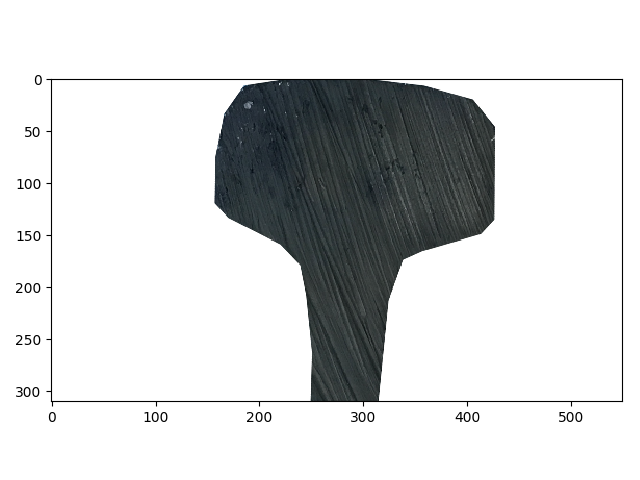
\includegraphics[width=0.75\textwidth]{images/up}}
     \vfill
     \subfloat[Rotated]{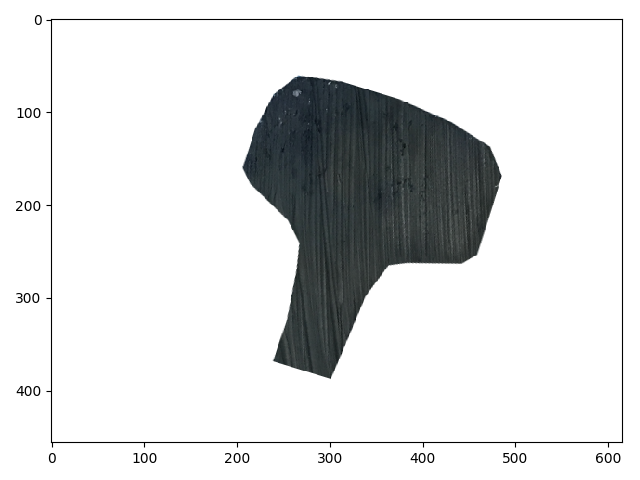
\includegraphics[width=0.75\textwidth]{images/rotated_up}}
     \caption{Rotation perpendicular to X-axis}
     \label{fig:image_rotation}
\end{figure}

\begin{figure}[H]
     \centering
     \subfloat[Pattern code]{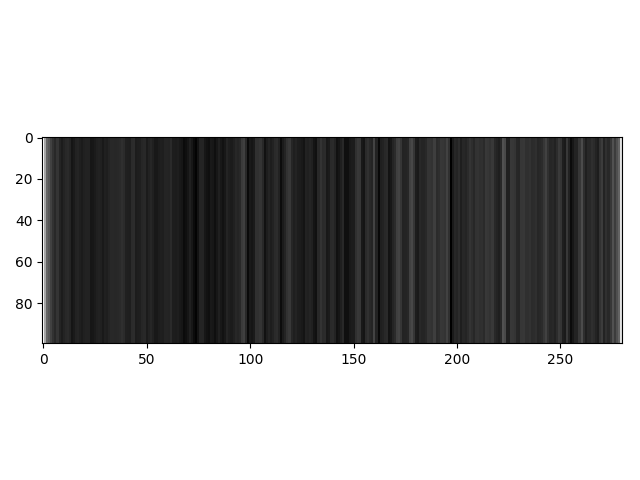
\includegraphics[width=0.75\textwidth]{images/rotated_up_code}}
     \vfill
     \subfloat[Corresponding histogram]{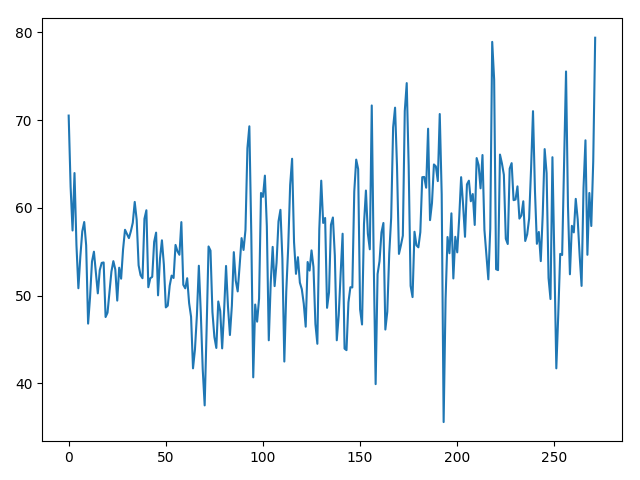
\includegraphics[width=0.75\textwidth]{images/rotated_up_hist}}
     \caption{Code and its' histogram}
     \label{fig:code_with_histogram}
\end{figure}

\paragraph{}
Figure \ref{fig:image_rotation} presents the already-extracted upper half of the rail surface before and after rotation. This procedure outputs an image, where the "barcode" lines are aligned perpendicular to the X-axis. 

\paragraph{}
After that, figure \ref{fig:code_with_histogram} shows the code that was read from the image (it actually is a single-row vector, only for plotting purposes that row is multiplied and we can see the code) and the histogram that corresponds to its grayscale values.

\paragraph{}
The whole process of mapping the rail image to a barcode (single-row vector) was to reduce the dimensionality of the task on hand. Now it was just a matter of finding a smart way to compare this vectors and assign them some similarity score. This is where the histogram that was computed on the earlier stages comes in handy. There are already known methods of comparing them and one that was performing well was chosen in the comparison algorithm implementation.

\paragraph{}
In order to actually compare two histograms $H$ (equation \ref{eq:hist_H}) and $G$ (equation \ref{eq:hist_G}) with the same number of bins\footnote{$h_1$ is the number of elements in the first bin, $h_2$ in the second bin, e.t.c. The same holds true for $g_1$, $g_2$, \dots, $g_n$}:

\begin{equation}
	H = \{h_1, h_2, \dots, h_n\}
	\label{eq:hist_H}
\end{equation}

\begin{equation}
	G = \{g_1, g_2, \dots, g_n\}
	\label{eq:hist_G}
\end{equation}
a metric $d(H, G)$ is to be chosen. The algorithm uses \textbf{correlation} (which is selected by using \textbf{CV\_HISTCMP\_CORREL} flag for OpenCV's \textit{compareHist} function). The metric is then defined as:
\begin{equation}
	d(H, G) = \frac{\sum_{i=1}^{n}(h_i - \bar{h})(g_i - \bar{g})}{\sqrt{\sum_{i=1}^{n}(h_i - \bar{h})^2 \sum_{i=1}^{n}(g_i - \bar{g})^2}}
	\label{eq:hist_comparison}
\end{equation}
where:
\begin{equation}
	\bar{h} = \frac{1}{n} \sum_{i=1}^{n} h_i
\end{equation}
and:
\begin{equation}
	\bar{g} = \frac{1}{n} \sum_{i=1}^{n} g_i
\end{equation}
while $n$ being the total number of bins in histogram.

\paragraph{Example}
Let us now look at a concrete example of comparing two histograms. Suppose we have two input arrays



\begin{equation*}
	A_H = [0,0,1,1,1,1,2,2,2]
\end{equation*}

and

\begin{equation*}
	A_G = [0,0,1,1,1,2,2,2,2]
\end{equation*}

\paragraph{}
Table \ref{tab:histogram_comparison} shows count of different values in both input arrays, whereas figure \ref{fig:histogram_comparison_plot} presents plots of those histograms.

\begin{table}[H]
    \centering
	\begin{spacing}{1.5}    
    \begin{tabular}{|l|l|l|}
        \hline
        \cellcolor{gray} & \textbf{$H$} & \textbf{$G$} \\ [0.5ex]
        \hline\hline
        \textbf{0} & 2 & 2 \\ [0.5ex]
        \hline
        \textbf{1} & 4 & 3 \\ [0.5ex]
        \hline
        \textbf{2} & 3 & 4 \\ [0.5ex]
        \hline
    \end{tabular}
    \end{spacing}
    \caption{Histograms for $A_H$ ($H$) and $A_G$ ($G$)}
    \label{tab:histogram_comparison}
\end{table}

\begin{figure}[H]
     \centering
     \subfloat[]{
\includegraphics[width=0.45\textwidth]{images/histogram_1}}
     \qquad
     \subfloat[]{
\includegraphics[width=0.45\textwidth]{images/histogram_2}}
     \caption{Plots of histograms $H$ (a) and $G$ (b)}
     \label{fig:histogram_comparison_plot}
\end{figure}

The histograms can then be represented as follows:

\begin{equation*}
	H = \{h_1, h_2, h_3\} = \{2, 4, 3\}
\end{equation*}

and:

\begin{equation*}
	G = \{g_1, g_2, g_3\} = \{2, 3, 4\}
\end{equation*}

The average values $\bar{h}$ and $\bar{g}$ can now be computed:

\begin{equation}
	\bar{h} = \frac{1}{3} * (2 + 4 + 3) = \frac{1}{3} * 9 = 3
	\label{eq:h_1_avg}
\end{equation}

\begin{equation}
	\bar{g} = \frac{1}{3} * (2 + 3 + 4) = \frac{1}{3} * 9 = 3
	\label{eq:h_2_avg}
\end{equation}

Then we should insert values from table \ref{tab:histogram_comparison} and averages from the equation \ref{eq:h_1_avg} and from the equation \ref{eq:h_2_avg} into the formula for computing the metric of histogram comparison (the equation \ref{eq:hist_comparison}):

\begin{equation}
\begin{aligned}
	d(H_1, H_2) = \frac{(2-3)*(2-3) + (4-3)*(3-3) + (3-3)*(4-3)}{\sqrt{((2-3)^2 + (4-3)^2 + (3-3)^2)((2-3)^2 + (3-3)^2 + (4-3)^2)}} = \\ \\ 
	= \frac{(-1) * (-1) + 1 * 0 + 0 * 1}{\sqrt{((-1)^2 + 1^2 + 0^2) * ((-1)^2 + 0^2 + 1^2)}} 
	= \frac{1 + 0 + 0}{\sqrt{(1+1+0)*(1+0+1)}} = \\ \\
	= \frac{1}{\sqrt{2 * 2}} = \frac{1}{\sqrt{4}} = \frac{1}{2}
	\label{eq:comparison_result}
\end{aligned}
\end{equation}

\paragraph{}
The result of histogram comparison from equation \ref{eq:comparison_result} can be confirmed with the code listing \ref{lst:comparison_result}:

\begin{lstlisting}[language=Python, caption=Histogram comparison in Python, label={lst:comparison_result},basicstyle={\ttfamily}]
import cv2
import numpy as np

a1 = np.asarray([0,0,1,1,1,1,2,2,2])
a2 = np.asarray([0,0,1,1,1,2,2,2,2])

h1, _ = np.histogram(a1, bins=3, range=(0, 2))
h2, _ = np.histogram(a2, bins=3, range=(0, 2))

d = cv2.compareHist(h1, h2, cv2.HISTCMP_CORREL)
\end{lstlisting}

\paragraph{}
The histograms that are obtained for two rail images may actually differ in sizes and for the aforementioned comparison method they need to be same-sized. That is why we take the shorter histogram and slide it over the longer one, do the comparison one offset at a time and take the highest from the output values.

\begin{algorithm}
	\begin{spacing}{1.5}
	\begin{algorithmic}[1]
		\Function{compareHist}{$h1, h2$}	
			\If{$\textbf{length}(h1) == \textbf{length}(h2)$}
				\State \textbf{return} $cv2.compareHist(h1, h2, cv2.HISTCMP\_CORREL)$
			\ElsIf{$\textbf{length}(h1) > \textbf{length}(h2)$}
				\State \textbf{return} $\textbf{maxHistComparison}(h1, h2)$
			\Else
				\State \textbf{return} $\textbf{maxHistComparison}(h2, h1)$
			\EndIf
		\EndFunction
	\end{algorithmic}
	\end{spacing}
	\caption{Histogram comparison}
	\label{alg:hist_comparison}
\end{algorithm}

\begin{algorithm}
	\begin{spacing}{1.5}
	\begin{algorithmic}[1]
		\Function{maxHistComparison}{$longer, shorter$}	
			\State $\text{len\_shorter} \gets \textbf{length}(shorter)$
			\State $\text{diff} \gets \textbf{length}(longer) - \textbf{length}(shorter)$
			\State $\text{max\_result} \gets -1$
			\For{$\text{offset} \gets 0\ \textbf{to}\ \text{diff}$}
				\State $\text{result} \gets \textbf{compareHist}(longer[\text{offset : offset + len\_shorter}], shorter)$
				\State $\text{max\_result} \gets \textbf{max}(\text{max\_result, result})$
			\EndFor
			\State \textbf{return} $\text{max\_result}$
		\EndFunction
	\end{algorithmic}
	\end{spacing}
	\caption{Histogram comparison - helper function}
	\label{alg:hist_comparison_helper}
\end{algorithm}

\paragraph{}
Let us now look at the Algorithm \ref{alg:hist_comparison_helper}. In lines 2 and 3 the length of the shorter histogram is obtained as well as the difference in sizes between two input histograms. The variable $max\_result$ is then set to -1 to notify that no actual check was yet performed. And then the loop, in lines 5 through 8, performs histogram comparison with increasing offset on the longer histogram and assigns to $max\_result$ the maximum of the actual $max\_result$ and the new comparison result. Finally, in line 9 the overall maximum result is returned.

\paragraph{}
The final result of the comparison, as already mentioned before, takes into consideration some slight differences in the dominant angle detection (does so be applying some artificial rotations in the process) and also for the size of the code (because the smaller one is searched through the larger one). Such a result - the similarity score - is then simply compared to a threshold value. If this outcome is greater than that threshold we can say that both images represent rail with the same code, which in our case means it represents the same rail. Otherwise, we can say that those images represent two different rails.

\subsection{Importance of the image angle} \label{subsect:angle_importance}
\paragraph{}
As it later turned out, the angle under which an image was taken plays a very significant role. That is why in \autoref{chap:results} results are split into angle buckets to point out this importance. Thus, if this solution was to be implemented in production usage, a consistent angle would be required to ensure the best possible performance of the presented algorithm.










